\documentclass{article}
\RequirePackage{ifpdf}
%\usepackage[accepted]{icml2013}
\usepackage[accepted]{icml2014}
\usepackage[algo2e,ruled]{algorithm2e}
%\usepackage{natbib,booktabs}
\usepackage{natbib}
\usepackage{graphicx} % more modern
\usepackage{hyperref,multirow,float}
\usepackage{paralist,xspace}
\usepackage{subfigure}
\usepackage{amsmath}
\usepackage{steinmetz}


\icmltitlerunning{A functional approximation based distributed learning algorithm}

%
% If your paper is accepted, change the options for the package
% aistats2012 as follows:
%
%\usepackage[accepted]{aistats2012}
%
% This option will print headings for the title of your paper and
% headings for the authors names, plus a copyright note at the end of
% the first column of the first page.
\usepackage{amsmath,amssymb}

\begin{document}


% If your paper is accepted and the title of your paper is very long,
% the style will print as headings an error message. Use the following
% command to supply a shorter title of your paper so that it can be
% used as headings.
%

% If your paper is accepted and the number of authors is large, the
% style will print as headings an error message. Use the following
% command to supply a shorter version of the authors names so that
% they can be used as headings (for example, use only the surnames)
%

%\runningauthor{Dhruv Mahajan, S. Sundararajan, S. Sathiya Keerthi, L\'{e}on Bottou}


\twocolumn[
\icmltitle
{A Functional Approximation Based Distributed Learning Algorithm}

\icmlauthor{Dhruv Mahajan}{dhrumaha@microsoft.com}
\icmladdress{Microsoft Research India,
            Bangalore, India}

\icmlauthor{S. Sathiya Keerthi}{keerthi@microsoft.com}
\icmladdress{Cloud and Information Services Lab,
            Microsoft Corporation, Mountain View, USA}

\icmlauthor{S. Sundararajan}{ssrajan@microsoft.com}
\icmladdress{Microsoft Research India,
            Bangalore, India}

\icmlauthor{L\'{e}on Bottou}{leonbo@microsoft.com}
\icmladdress{Microsoft Research,
            New York, USA}


\vskip 0.3in
]

\author{Dhruv Mahajan, S. Sundararajan, S. Sathiya Keerthi}

\begin{abstract}
This paper gives a novel approach to the distributed training of linear classifiers. At each iteration, the nodes minimize approximate objective functions and combine the resulting minimizers to form a descent direction to move. The method is shown to have $O(\log(1/\epsilon))$ time convergence. The method can be viewed as an iterative parameter mixing method. A special instantiation yields a parallel stochastic gradient descent method with strong convergence. When communication times between nodes are large, our method is much faster than the SQM method, which uses distributed computation only for function and gradient calls.
\end{abstract}


%\maketitle

\def\grad{\nabla}
\def\wtilde{\tilde{w}}
\def\Cone{{\cal{C}}^1}
\def\kappap{\kappa^\prime}
\def\Lhat{\hat{L}}
\def\fhat{\hat{f}}
\def\what{\hat{w}}
\def\dhat{\hat{d}}
\def\mysgn{\operatorname{sgn}}
\def\ftilde{\tilde{f}}
\def\khat{\hat{k}}
\def\defs{\stackrel{\text{def}}{=}}
\def\vhat{\hat{v}}

\def\ttilde{\tilde{t}}
\def\that{\hat{t}}
\def\tstar{t^\star}

\section{Introduction}
\label{intro}

Consider the batch learning of a linear classifier with a differentiable convex loss function and an $L_2$ regularizer. This involves the minimization of a convex differentiable objective function $f(w)$ where $w$ is the weight vector. The minimization is usually performed using an iterative descent method in which an iteration starts from a point $w^r$, computes a direction $d^r$ that satisfies
\begin{equation}
\mbox{{\small\bf sufficient angle of descent:}}\; \phase{-g^r, d^r} \le \theta \label{angle}
\end{equation}
where $g^r=g(w^r)$, $g(w)=\grad f(w)$, $\phase{a,b}$ is the angle between vectors $a$ and $b$, and $0 \le \theta < \pi/2$, and then performs a line search along the direction $d^r$ to find the next point, $w^{r+1}=w^r+t d^r$. Let $w^\star=\arg\min_w f(w)$. A key contribution of this paper is the proof that, when $f$ is convex and satisfies some additional weak assumptions, the method has global linear rate of convergence ({\it glrc})\footnote{We say a method has {\it glrc} if $\exists$ $0<\delta<1$ such that $(f(w^{r+1})-f(w^\star)) \le \delta (f(w^r)-f(w^\star))\;\forall r$.} and so it finds a point $w^r$ satisfying $f(w^r)-f(w^\star)\le\epsilon$ in $O(log(1/\epsilon))$ iterations. {\it The main theme of this paper is that the flexibility offered by this method with good convergence properties allows us to build a class of useful distributed learning methods.}

Let us consider large scale learning in a distributed setting in which examples are partitioned over a number of computing nodes. Take one of the most effective distributed methods, viz., SQM (Statistical Query Model)~\cite{chu2006,agarwal2011}, which is a batch, gradient-based descent method. The gradient is computed in a distributed way with each node computing the gradient component corresponding to its set of examples. This is followed by an aggregation of the components. Consider a scenario in which the communication time between nodes is large relative to the computation time in each node.\footnote{This is the case when feature dimension is huge. Many applications gain performance when the feature space is expanded, say, via feature combinations, explicit expansion of nonlinear kernels etc.} In such a scenario, it is useful to ask: {\bf Q1.} {\it Can we do more computation in each node so that the number of communication passes is decreased, thus reducing the total computing time?}
%We will show that this question can be answered positively by using the iterative descent method suitably.

There have been some efforts in the literature to reduce the amount of communication. In these methods, the current $w^r$ is first passed on to all the nodes. Then, each node $p$ forms an approximation $\ftilde_p$ of $f$ using only its examples, followed by several optimization iterations (local passes over its examples) to decrease $\ftilde_p$ and reach a point $w_p$. The $w_p\;\forall p$ are averaged to form the next iterate $w^{r+1}$. One can stop after just one major iteration (going from $r=0$ to $r=1$); such a method is referred to as {\it parameter mixing (PM)}~\cite{mann2009}. Alternatively, one can do many major iterations; such a method is referred to as {\it iterative parameter mixing (IPM)}~\cite{hall2010}. Convergence theory for such methods is inadequate~\cite{mann2009, mcdonald2010}, which prompts us to ask: {\bf Q2.} {\it Is it possible to devise an IPM method that produces $\{w^r\} \rightarrow w^\star$?}

For large scale learning on a single machine, it is now well established that example-wise methods\footnote{These methods update $w$ after scanning each example.} such as stochastic gradient descent (SGD) and its variations~\cite{bottou2010, johnson2013} and dual coordinate ascent~\cite{hsieh2008} are much faster than batch gradient-based methods. However, example-wise methods are inherently sequential. If one employs a method such as SGD as the local optimizer for $\ftilde_p$ in PM/IPM, the result is, in essence, a parallel SGD method. However, convergence theory for such a method is limited, even that requiring a complicated analysis~\cite{zinkevich2010}. Thus, we ask: {\bf Q3.} {\it Can we form a parallel SGD method with strong convergence properties?}

We make a novel and simple use of the iterative descent method mentioned at the beginning of this section to design a distributed algorithm that answers Q1-Q3 positively. The main idea is to use distributed computation for generating a good search direction $d^r$ and not just for forming the gradient as in SQM. At iteration $r$, let us say each node $p$ has the current iterate $w^r$ and the gradient $g^r$. This information can be used together with the examples in the node to form a function $\fhat_p(\cdot)$ that approximates $f(\cdot)$ and satisfies $\grad\fhat_p(w^r)=g^r$. One simple and effective suggestion is:
\begin{equation}
\fhat_p(w)=f_p(w)+(g^r - \nabla f_p(w^r))\cdot(w-w^r)
\label{sugg1}
\end{equation}
where $f_p$ is the part of $f$ that does not depend on examples outside node $p$. In section~\ref{distr} we give other suggestions for forming $\fhat_p$. Now $\fhat_p$ can be optimized within node $p$ using any method ${\cal M}$ which has {\it glrc}, e.g., Trust region method, L-BFGS, etc. There is no need to optimize $\fhat_p$ fully. We show (see section~\ref{distr}) that, in a constant number of local passes over examples in node $p$, an approximate minimizer $w_p$ of $\fhat_p$ can be found such that the direction $d_p=w_p-w^r$ satisfies the sufficient angle of descent condition, (\ref{angle}). The set of directions generated in the nodes, $\{d_p\}$ can be averaged to form the overall direction $d^r$ for iteration $r$. Note that $d^r$ also satisfies (\ref{angle}). The result is an overall distributed method that finds a point $w$ satisfying $f(w)-f(w^\star)\le\epsilon$ in $O(\log (1/\epsilon))$ time. This answers {\bf Q2}.

The method also reduces the number of distributed passes over the examples compared with SQM, thus also answering {\bf Q1}. The intuition here is that, if each $\fhat_p$ is a good approximation of $f$, then $d^r$ will be a good global direction for minimizing $f$ at $w^r$, and so the method will move towards $w^\star$ much faster than SQM.
As one special instantiation of our distributed method, we can use, for the local optimization method ${\cal M}$, any variation of SGD with {\it glrc} (in expectation), e.g., the one in Johnson \& Zhang~\yrcite{johnson2013}. For this case, our method has $O(\log (1/\epsilon))$ time convergence in a probabilistic sense (Mahajan et al. NIPS workshop paper). The result is a strongly convergent parallel SGD method, which answers {\bf Q3}. An interesting side observation is that, the single machine version of this instantiation is very close to the variance-reducing SGD method in Johnson \& Zhang~\yrcite{johnson2013}.


%In section~\ref{expts} we demonstrate this via experiments on distributed implementations of the methods using {\it AllReduce} on Hadoop.

%The set up described above can also be used to to devise a method which fills an important gap in the distributed learning literature. Let us first describe this gap before describing our solution. For large scale learning on a single machine, it is now well established that example-wise methods\footnote{These methods update $w$ after scanning each example.} such as stochastic gradient descent (SGD) and its variations~\cite{bottou2010, johnson2013} and dual coordinate ascent~\cite{hsieh2008} are much faster than batch gradient-based methods. However, example-wise methods are inherently sequential. There have been attempts to parallelize them using the following idea: pass the current $w^r$ to all nodes, in each node $p$ apply one or more epochs of SGD on its examples to generate $w_p$, and then average the $w_p$ using a {\it Reduce} operation to form $w^{r+1}$. One can stop such {\it parameter mixing} methods after a single iteration~\cite{zinkevich2010, mann2009} (going from $r=0$ to $r=1$) or do several iterations~\cite{hall2010, mcdonald2010}; however, establishing convergence of such methods is limited as well as hard.

%Let us now briefly describe our solution. Suppose, in our distributed method described earlier, we form $\fhat_p$ using (\ref{sugg1}), use a SGD method as the choice for $\cal{M}$ to minimize $\fhat_p$, and run several epochs of SGD updates over the examples of node $p$, then a $w_p$ can be generated so that $d_p=w_p-w^r$ satisfies (\ref{angle}). Averaging the $d_p$ to generate $d^r$ followed by line search completes an iteration. The resulting instantiation of Algorithm~\ref{GD} has good convergence properties  and is a nice parallelization of SGD. The ability to inject an example-wise method in a batch method is interesting as well as a demonstration of the flexibility offered by our approach to large scale distributed learning. Another interesting observation is that, the single machine version of this instantiation is very close to a recently proposed variance-reducing SGD method~\cite{johnson2013}.

In summary, the paper makes the following contributions. (1) For convex $f$ we establish {\it glrc} for a general iterative descent method. (2) We propose a distributed learning algorithm that: (a) converges in $O(\log (1/\epsilon))$ time, thus leading to an IPM method with strong convergence; (b) is more efficient than SQM when communication times are high; and (c) flexible in terms of the local optimization method ${\cal M}$ that can be used in the nodes. (3) We give an effective parallelization of SGD with good theoretical support and make connections with a recently proposed variance-reducing SGD method. 

Experiments validate our theory as well as show the benefits of our method for large dimensional datasets where communication is the bottleneck. We conclude with a discussion on unexplored possibilities for extending our distributed learning method in section~\ref{disc}.

%We close this section with a brief discussion of works related to this paper.

%\noindent {\bf Related work.} Let us begin with papers related to the general descent method and its convergence.

\section{Convergence of the descent method}
\label{general}

Let $f\in\Cone$, the class of continuously differentiable functions\footnote{It would be interesting future work to extend all the theory developed in this paper to non-differentiable convex functions, using sub-gradients.}, $f$ be convex, and the gradient $g$ satisfy the following assumptions.

{\bf A1.} $g$ is Lipschitz continuous, i.e., $\exists$ $L>0$ such that
$\|g(w)-g(\wtilde)\| \le L \|w-\wtilde\| \;\;\; \forall \; w, \wtilde$.

{\bf A2.} $\exists$ $\sigma >0$ such that
$(g(w)-g(\wtilde))\cdot(w-\wtilde) \ge \sigma \|w-\wtilde\|^2  \;\;\; \forall \; w, \wtilde$.

A1 and A2 are essentially second order conditions: if $f$ happens to be twice continuously differentiable, then $L$ and $\sigma$ can be viewed as upper and lower bounds on the eigenvalues of the Hessian of $f$. A convex function $f$ is said to be $\sigma$- strongly convex if $f(w)-\frac{\sigma}{2} \|w\|^2$ is convex. In machine learning, all convex risk functionals in $\Cone$ having the $L_2$ regularization term, $\frac{\lambda}{2} \|w\|^2$ are $\sigma$- strongly convex with $\sigma=\lambda$. It can be shown~\cite{smola2008} 
%(see (3.18) there)
that, if $f$ is $\sigma$-strongly convex, then $f$ satisfies assumption A2.

Let $f^r=f(w^r)$, $g^r=g(w^r)$ and $w^{r+1}=w^r+t d^r$. Consider the following standard line search conditions.
\begin{eqnarray}
\mbox{{\small\bf Armijo:}}\; & f^{r+1} \le f^r + \alpha g^r\cdot(w^{r+1}-w^r) \label{ag} \\
\mbox{{\small\bf Wolfe:}}\;  & g^{r+1}\cdot d^r \ge \beta g^r\cdot d^r \label{wolfe}
\end{eqnarray}
where $0<\alpha<\beta<1$.

\begin{algorithm2e}
\caption{Descent method for $f$\label{GD}}
Choose $w^0$\;
\For{$r=0,1 \ldots$}{
1. Exit if $g^r=0$\;
2. Choose a direction $d^r$ satisfying (\ref{angle})\;
3. Do line search to choose $t>0$ so that $w^{r+1}=w^r+td^r$ satisfies the Armijo-Wolfe conditions (\ref{ag}) and (\ref{wolfe})\;
}
\end{algorithm2e}
Let us now consider the general descent method in Algorithm~\ref{GD} for minimizing $f$. The following result shows that the algorithm is well-posed. A proof is given in the appendix.

%Standard results in optimization~\cite{dennis1996} (see Theorem 6.3.2) can be easily modified to show that there always exists an interval of $t$ values over which (\ref{wolfe}) and (\ref{ag}) hold.

{\bf Lemma 1.} Suppose $g^r\cdot d^r<0$.
Then $\{ t: $ (\ref{ag}) and (\ref{wolfe}) hold for $w^{r+1}=w^r+td^r\} = [t_\beta,t_\alpha]$, where $0<t_\beta<t_\alpha$, and $t_\beta$, $t_\alpha$ are the unique roots of
\begin{eqnarray}
g(w^r+t_\beta d^r)\cdot d^r = \beta g^r\cdot d^r, \label{tbeta} \\
f(w^r+t_\alpha d^r) = f^r + t_\alpha \alpha g^r\cdot d^r, \;\; t_\alpha>0. \label{talpha}
\end{eqnarray}

%If $\alpha$ is chosen very small, say $\alpha=10^{-4}$ and $\beta$ close to 1, say $0.99$, then this interval becomes large and it is easy to locate a $t$ satisfying the two conditions. (We need to say a bit more here, e.g., give good starting $t$ values and a clean line search algorithm that works and is also efficient. See section~\ref{lsearch} for some ideas for bracketing the minimum in the line search.)

{\bf Theorem 2.} Let $w^\star=\arg\min_w f(w)$ and $f^\star=f(w^\star)$.\footnote{Assumption A2 implies that $w^\star$ is unique.} Then $\{w^r\}\rightarrow w^\star$. Also, we have {\it glrc}, i.e., $\exists$ $\delta$ satisfying $0<\delta<1$ such that
$(f^{r+1} - f^\star) \le \delta\, (f^r-f^\star) \; \forall \; r\ge 0$,
and, $f^r-f^\star\le\epsilon$ is reached after at most
$\frac{\log ((f^0-f^\star)/\epsilon)}{\log(1/\delta)}$
iterations. An upper bound on $\delta$ is $(1 - 2\alpha(1-\beta)\frac{\sigma^2}{L^2} \cos^2\theta)$.\footnote{The actual rate of convergence is usually a lot better, and it depends much on the method used for choosing $d^r$.}

A proof of Theorem 2 is given in the appendix. If one is interested only in proving convergence, it is easy to establish under the assumptions made; such theory goes back to the classical works of Wolfe~\yrcite{wolfe1969, wolfe1971}. But proving {\it glrc} is harder. There exist proofs for special cases such as the gradient descent method~\cite{boyd2004}. The {\it glrc} result in Wang \& Lin~\yrcite{wang2013} is only applicable to descent methods that are ``close" (see equations ($7$) and ($8$) in~\cite{wang2013}) to the gradient descent method. Though Theorem 2 is not entirely surprising, as far as we know, such a result does not exist in the literature.

\section{Distributed training}
\label{distr}

Let $\{x_i,y_i\}$ be the training set associated with a binary classification problem ($y_i\in\{1,-1\}$). Consider a linear classification model, $y=\mysgn(w^Tx)$. Let $l(w\cdot x_i,y_i)$ be a continuously differentiable loss function that has Lipschitz continuous gradient. This allows us to consider loss functions such as least squares, logistic loss and squared hinge loss. Hinge loss is not covered by our theory since it is non-differentiable.

Suppose the data is distributed in $P$ nodes. Let: $I_p$ be the set of indices $i$ such that $(x_i,y_i)$ sits in the $p$-th node; $L_p(w) = \sum_{i\in I_p} l(w;x_i,y_i)$ be the total loss associated with node $p$; and, $L(w)=\sum_p L_p(w)$ be the total loss over all nodes. Our aim is to to minimize the regularized risk functional $f(w)$ given by
\begin{equation}
f(w) = \frac{\lambda}{2} \|w\|^2 + L(w) = \frac{\lambda}{2} \|w\|^2 + \sum_p L_p(w)
\label{risk}
\end{equation}
where $\lambda>0$ is the regularization constant. It is easy to check that $g=\grad f$ is Lipschitz continuous.

Our distributed method is based on the descent method in Algorithm~\ref{GD}. We use a master-slave architecture.\footnote{An {\it AllReduce} arrangement of nodes~\cite{agarwal2011} may also be used.} Let the examples be partitioned over $P$ slave nodes. Distributed computing is used to compute the gradient $g^r$ as well as the direction $d^r$.  In the $r$-th iteration, let us say that the master has the current $w^r$ and gradient $g^r$. One can communicate these to all $P$ (slave) nodes. The direction $d^r$ is formed as follows. Each node $p$ constructs an approximation of $f(w)$ using only information that is available in that node, call it $\fhat_p(w)$, and (approximately) optimizes it (starting from $w^r$) to get the point $w_p$. Let $d_p=w_p-w^r$. Then $d^r$ is chosen to be any convex combination of $d_p\;\forall p$.

Our method offers great flexibility in choosing $\fhat_p$ and the method used to optimize it. We only require $\fhat_p$ to satisfy the following.

{\bf A3.} $\fhat_p$ is $\sigma$-strongly convex, has Lipschitz continuous gradient and satisfies {\it gradient consistency at $w^r$:} $\grad\fhat_p(w^r)=g^r$.

Below we give ways of forming $\fhat_p$. The $\sigma$-strongly convex condition is easily taken care of by making sure that the $L_2$ regularizer is a part of $\fhat_p$. This condition implies that
\begin{equation}
\fhat_p(w_p) \ge \fhat_p(w^r) + \grad\fhat_p(w^r)\cdot (w_p-w^r) + \frac{\sigma}{2} \|w_p-w^r\|^2
\label{fhatsig}
\end{equation}
The gradient consistency condition is motivated by the need to satisfy the angle condition (\ref{angle}). Since $w_p$ is obtained by starting from $w^r$ and optimizing $\fhat_p$, it is reasonable to assume that $\fhat_p(w_p)<\fhat_p(w^r)$. Using these in (\ref{fhatsig}) gives $-g^r\cdot d_p > 0$. Since $d^r$ is a convex combination of the $d_p$ it follows that $-g^r\cdot d^r > 0$. Later we will formalize this to yield (\ref{angle}) precisely.

A natural way of choosing the approximating functional $\fhat_p$ is
\begin{equation}
\fhat_p(w) = \frac{\lambda}{2} \|w\|^2 + L_p(w) +\Lhat_p(w)
\label{riskapp}
\end{equation}
where $\Lhat_p(w)$ is an approximation of $L(w)-L_p(w)=\sum_{q\not= p} L_q(w)$, but one that does not explicitly require any examples outside node $p$. To satisfy A3 we only need $\Lhat_p$ to have Lipschitz continuous gradient; all other conditions are directly satisfied. A simple instance of $\Lhat_p$ is a linear function constructed using the gradient at $w^r$:
\begin{equation}
\Lhat_p(w) = (g^r - \lambda w^r-\grad L_p(w^r))\cdot(w-w^r)
\label{linapp}
\end{equation}
(The zeroth order term needed to get $f(w^r)=\fhat(w^r)$ is omitted because it is a constant that plays no role in the optimization.) There are other ways of forming an approximation $\Lhat_p(w)$. For example, one could add a second order term, $\frac{1}{2}(w-w^r)\cdot H(w-w^r)$ to the approximation in (\ref{linapp}) where $H$ is a positive semi-definite matrix; for $H$ we can use a diagonal approximation or keep a limited history of gradients and form a BFGS approximation of $L-L_p$.

%It is easy to check that the $\fhat_p$ given by (\ref{riskapp}) and (\ref{linapp}) satisfies the above conditions. It is worth noting that, due to the regularization term $\frac{\lambda}{2} \|w\|^2$, $f$ and $\fhat_p$ are $\sigma$-strongly convex, with $\sigma=\lambda$.

{\bf Convergence Theory.} The distributed method described above is an instance of Algorithm~\ref{GD} and so Theorem 2 can be used. However, obtaining $d^r$ requires the determination of the $w_p$ via minimizing $\fhat_p$. As already mentioned, it is not necessary for $w_p$ to be the minimizer of $\fhat_p$; we only need to find $w_p$ such that the direction $d_p=w_p-w^r$ satisfies (\ref{angle}). The angle $\theta$ needs to be chosen right. Let us discuss this first. Let $\what_p^\star$ be the minimizer of $\fhat_p$. It can be shown (see appendix A) that $\phase{\what_p^\star-w^r,-g^r} \le \cos^{-1}\frac{\sigma}{L}$. To allow for $w_p$ being an approximation of $\what_p^\star$, we choose $\theta$ such that
\begin{equation}
\frac{\pi}{2} > \theta > \cos^{-1} \frac{\sigma}{L}
\label{thetadef}
\end{equation}
The following result shows that if an optimizer with {\it glrc} is used to minimize $\fhat_p$, then, only a constant number of iterations is needed to satisfy the sufficient angle of descent condition.

{\bf Lemma 3.} Assume $g^r\not=0$. Suppose we minimize $\fhat_p$ using an optimizer ${\cal M}$ that starts from $v^0=w^r$ and generates a sequence $\{v^k\}$ having {\it glrc}, i.e.,
$\fhat_p(v^{k+1}) - \fhat_p^\star \le \delta (\fhat_p(v^k) - \fhat_p^\star)$,
where $\fhat_p^\star = \fhat_p(\what_p^\star)$. Then, there exists $\khat$ (which depends only on $\sigma$ and $L$) such that
$\phase{-g^r,v^k-w^r} \le \theta \;\; \forall k\ge \khat$.

Lemma 3 can be combined with Theorem 2 to yield the following convergence theorem.

{\bf Theorem 4.} Suppose $\theta$ satisfies (\ref{thetadef}), ${\cal M}$ is as in Lemma 3 and, in each iteration $r$ and for each $p$, $\khat$ or more iterations of ${\cal M}$ are applied to minimize $\fhat_p$ (starting from $w^r$) and get $w_p$. Then the distributed method converges to a point $w$ satisfying $f(w)-f(w^\star)\le\epsilon$ in $O(\log(1/\epsilon))$ time.

%{\bf Leon's comments to go here.} Proofs of the above results are given in appendix A. The bound on rate of convergence derived there should not be interpreted as the actual rates associated with our method. etc.

{\bf Related work.}
As already mentioned in section~\ref{intro} our distributed method can be viewed as an IPM method, but one which has strong convergence properties.

The ADMM method~\cite{Boyd2011}, like our method, solves approximate problems in the nodes and iteratively reaches the full batch solution. But it has the following disadvantages: (a) it does not have {\it glrc}; (b) the approximation problems are dictated by the ADMM formulation and so there is little flexibility; (c) the approximation problems need to be solved precisely; and (d) its efficiency is sensitive to the choice of the penalty parameter which is problem dependent.

{\bf Practical implementation.} Going with the practice in numerical optimization, we replace (\ref{angle}) by the condition, $-g^r\cdot d^r > 0$ and use $\alpha=10^{-4}$, $\beta=0.9$ in (\ref{ag}) and (\ref{wolfe}). We terminate Algorithm~\ref{GD} when $\|g^r\|\le \epsilon_g\|g^0\|$ is satisfied at some $r$. Let us take line search next. On $w=w^r+t d^r$, the loss has the form $l(z_i+te_i,y_i)$ where $z_i=w^r\cdot x_i$ and $e_i=d^r\cdot x_i$. Once we have computed $z_i\;\forall i$ and $e_i\;\forall i$, the distributed computation of $f(w^r+t d^r)$ and its derivative with respect to $t$ is cheap as it does not involve any computation involving the data, $\{x_i\}$. Thus many $t$ values can be explored cheaply. Since $d^r$ is determined by approximate optimization, $t=1$ is expected to give a decent starting point. We first identify an interval $[t_1,t_2]\subset [t_\beta,t_\alpha]$ (see Lemma 1) by starting from $t=1$ and doing forward and backward stepping. Then we check if $t_1$ or $t_2$ is the minimizer of $f(w^r+t d^r)$ on $[t_1,t_2]$; if not, we do several bracketing steps in $(t_1,t_2)$ to locate the minimizer approximately. Finally, when using method ${\cal M}$, we terminate it after a fixed number of steps, $\khat$. Algorithm 2 gives all the steps of the distributed method while also mentioning the distributed communications and computations involved.

\begin{algorithm2e}
\caption{Distributed method for minimizing $f$
{\it com:} communication; {\it cmp:} = computation; {\it agg:} aggregation}
Choose $w^0$\;
\For{$r=0,1 \ldots$}{
1. Compute $g^r$ ({\it com}: $w^r$; {\it cmp:} Two passes over data; {\it agg:} $g^r$); By-product: $\{z_i=w^r\cdot x_i\}$\;
2. Exit if $\|g^r\| \le \epsilon_g \|g^0\|$\;
3. \For{$p=1,\ldots,P$ (in parallel)}{
4.   Set $v^0=w^r$\;
5.   \For{$k=0,1,\ldots,\khat$}{
        6. Find $v^{k+1}$ using one iteration of ${\cal M}$\;
     }
     7. Set $w_p=v^{\khat+1}$\;
   }
8. Set $d^r$ as any convex combination of $\{w_p\}$ ({\it agg:} $w_p$)\;
9. Compute $\{e_i=d^r\cdot x_i\}$ ({\it comm:} $d^r$; {\it cmp:} One pass over data)\;
10. Do line search to find $t$ (for each $t$: {\it comm:} $t$; {\it cmp:} $l$ and $\partial l/\partial t$ {\it agg:} $f(w^r+t d^r)$ and its derivative wrt $t$)\;
11. Set $w^{r+1} = w^r+t d^r$\;
}
\end{algorithm2e}

{\bf Choices for ${\cal M}$.}
There are many good methods having (deterministic) {\it glrc}: L-BFGS, TRON~\cite{lin2008}, Primal coordinate descent~\cite{chang2008}, etc. One could also use methods with {\it glrc} in the expectation sense (in which case, convergence in Theorem 4 should also be interpreted in some probabilistic sense; see Mahajan et. al NIPS workshop paper for details). Recently suggested variants of SGD~\cite{leroux2012,johnson2013} are methods with such convergence. This particular instantiation of our distributed method yields a parallel SGD method with strong convergence properties, which, as already indicated in section~\ref{intro} (see Q3), fills a gap in the literature. In section~\ref{expts} we conduct experiments using TRON and the SVRG method in Johnson \& Zhang (2013).

{\bf{Connection with SVRG. }}
The connection of our method with the recently proposed SVRG method~\citep{johnson2013} is interesting. To show this, let us take the $\fhat_p$ in~(\ref{linapp}). Let $n_p=|I_p|$ be the number of examples in node $p$. Define $\psi_i(w) = n_p l(w\cdot x_i,y_i) + \frac{\lambda}{2} \|w\|^2$. It is easy to check that
\begin{equation}
\grad\fhat_p(w) = \frac{1}{n_p} \sum_{i\in I_p} ( \grad\psi_i(w) - \grad\psi_i(w^r) + g^r)
\label{psigrad}
\end{equation}
Thus, plain SGD updates applied to $\fhat_p$ has the form
\begin{equation}
w = w - \eta ( \grad\psi_i(w) - \grad\psi_i(w^r) + g^r)
\label{svrg}
\end{equation}
which is precisely the update in SVRG. In particular, the single node ($P=1$) implementation of our method using plain SGD updates for optimizing $\fhat_p$ is very close to the SVRG method.\footnote{Note the subtle point that applying SVRG method on $\fhat_p$ is different from doing (\ref{svrg}), which corresponds to plain SGD. It is the former that assures {\it glrc} (in expectation).} While Johnson \& Zhang~\yrcite{johnson2013} motivate the update in terms of variance reduction, we derive it from a functional approximation viewpoint.

{\bf Computation-Communication tradeoff.}
Compared to the SQM method (see section~\ref{intro}), our method does a lot more computation (optimize $\fhat_p$) in each node. On the other hand our method reaches a good solution using a much smaller number of outer iterations. Clearly, our method will be attractive for problems with high communication costs, e.g., problems with a large feature dimension. For a given distributed computing environment and specific implementation choices, it is easy to do a rough analysis to understand the conditions in which our method will be more efficient than SQM. Consider a distributed grid of nodes in an {\it AllReduce} tree. Let us use TRON for implementing SQM and SVRG for ${\cal M}$ in our method. Assuming that $T_{\rm SVRG}^{\rm outer}<3T_{\rm SQM}^{outer}$ (where $T_{\rm SVRG}^{\rm outer}$ and $T_{\rm SQM}^{outer}$ are the number of outer iterations required by SQM and our method with SVRG), we can do a rough analysis of the costs of SQM and our method (see appendix B for details) to show that our method will be faster when the following condition is satisfied.
\begin{equation}
\frac{nz}{m} \ll \frac{\gamma P \log_2 P}{2} \frac{T_{\rm SQM}^{\rm outer}}{\khat}
\label{comm}
\end{equation}
where: $nz$ is the number of nonzero elements in the data, i.e., $\{x_i\}$; $m$ is the feature dimension; $\gamma$ is the relative cost of communication to computation (e.g. $100-1000$); $P$ is the number of nodes; and $\khat$ is the number of inner iterations of our method.



\section{Experiments}
\label{expts}

\def\grad{\nabla}
\def\wtilde{\tilde{w}}
\def\Cone{{\cal{C}}^1}
\def\kappap{\kappa^\prime}
\def\Lhat{\hat{L}}
\def\fhat{\hat{f}}
\def\what{\hat{w}}
\def\dhat{\hat{d}}
\def\mysgn{\operatorname{sgn}}


%\def\kdd{{\it{kdd2010}}}
%\def\webspam{{\it{webspam}}}
%\def\url{{\it{url }}}
%\def\sqm{{\it{SQM }}}
%\def\hybrid{{\it{HYBRID }}}
%\def\oursvrg{{\it{FS-k }}}
%\def\ourtron{{\it{FT-k }}}


In this section, we demonstrate the effectiveness of our method on large dimensional data sets. We first discuss our experimental setup. We then show results
to validate the theory proposed in the paper. Finally, we compare our approach with existing distributed machine learning algorithms and clearly demonstrate scenarios under which our method performs better.

\subsection{Experimental Setup}
We run our experiments on a Hadoop cluster. Since iterations in traditional MapReduce are slower (because of job setup and disk access costs), as in Agarwal et al.~\yrcite{agarwal2011}, we build an AllReduce binary tree between the mappers\footnote{Note that we do not use the pipelined version and hence we incur an extra multiplicative $logP$ cost in communication.}. The communication bandwidth is $1 Gbps$ (gigabits per sec).  For functional approximation we use (\ref{riskapp}) and (\ref{linapp}). We use the Area under Precision-Recall Curve (AUPRC) and difference to the optimal function value as the evaluation criteria.\vspace{0.1in} \\

\begin{table}[ht]
\caption{Datasets} % title of Table
\centering % used for centering table
\begin{tabular}{c c c c c c c} % centered columns (4 columns)
\hline\hline %inserts double horizontal lines
Dataset & Examples & Features & Non-zeros\\ %[0.5ex] % inserts table
%heading
\hline 
{\it{kdd2010}} & $8.41M$ & $20.21M$ & 0.31B\\
{\it{url }} & $1.91M$ &  $3.23M$ &  0.22B\\
\hline 
\end{tabular}
\label{tab:params}
\end{table}

{\bf{Data Sets. }}We consider two well known large dimensional datasets: {\it{kdd2010}}  and {\it{url}}. Table~\ref{tab:params} shows the number of examples, features and nonzero feature values. We use these datasets mainly to illustrate the validity of theory, and its utility to distributed machine learning.\vspace{0.1in} \\
%illustration purpose only
{\bf{Methods for Comparison. }}We use the {\it{squared-hinge}} loss function with {\it{l2}}-regularization for all the experiments. We compare the following methods.

%\begin{itemize}
%\item {\bf{{\it{SQM}}: }}
\noindent{\bf{{\it{SQM: }}}}We use the Trust Region Newton method (TRON) proposed in Lin et al.~\yrcite{lin2008} and, do the gradient and Hessian computations in a parallel manner. We initialize the weight vector to zero and set all the parameters (except regularizer $\lambda$) to the values recommended in Lin et al.~\yrcite{lin2008}.
%\item {\bf{{\it{HYBRID}: }}

\noindent{\bf{{\it{HYBRID: }}}}We find a local weight vector per node by minimizing the local objective function (based only on the examples in that node) using one epoch of SGD~\cite{bottou2010}. (The optimal step size is chosen by running SGD on a subset of data.) We then average the weights from all the nodes and use the averaged weight vector to warm start {\it{SQM}}. Note that this method is same as that proposed in Agarwal et al.~\yrcite{agarwal2011} (except that they use the L-BFGS method instead of TRON).

\noindent{\bf{{\it{FS-k: }}}}Our algorithm with the SVRG method~\cite{johnson2013} used for solving the local optimization in every iteration. As suggested in~\cite{johnson2013}, we recalculate the batch gradient after every $5$ epochs (referred as outer iteration in the local optimization context). We run $k$ outer iterations of SVRG and show results for $k=8$ and $16$.

\noindent {\bf{{\it{FT-k: }}}}Our algorithm with TRON~\cite{lin2008} used for solving the local optimization. We stop the inner optimization after doing $k$ Hessian-vector multiplications. The results are shown for $k=50$ and $100$ for {\it{kdd2010}} and $k=25$ and $50$ for {\it{url}}.
%\end{itemize}

%In our algorithms we restricted the number of line search steps to $10$. Note that both TRON and SVRG are state of the art solvers and meet our condition of early stopping required in Theorem 4.

%choice of number of inner iterations is dependent on number of nodes
%say that do not use outer iterations
%ours is good global cnvergence and slow local movement vice versa for them
%wrt no. of nodes vs. ours
%tron vs. svrg

\begin{figure}[t]
\centering
\subfigure[{\it{kdd2010}} - 25 nodes]{
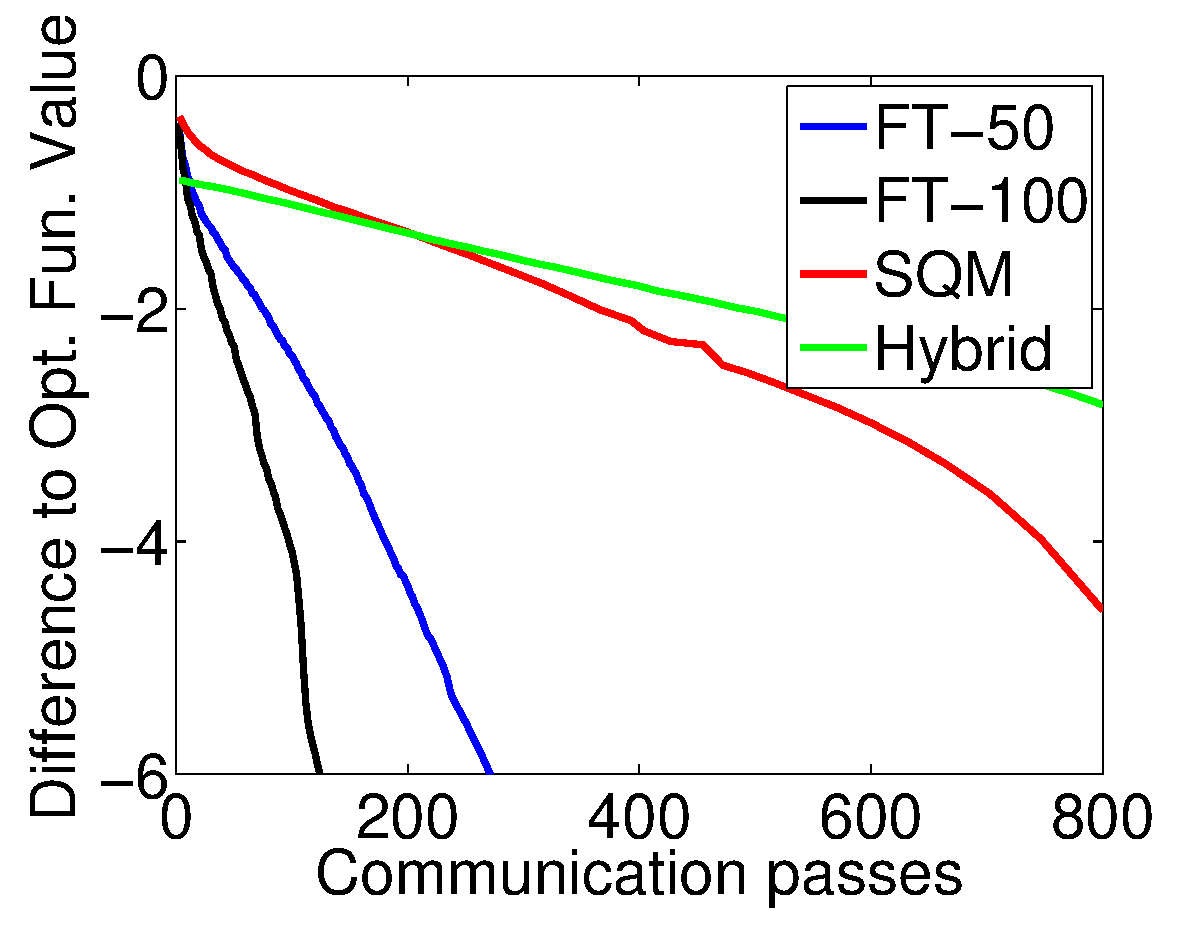
\includegraphics[width=0.46\linewidth]{figures/kddtron_25nodes_outeriters}
}
\subfigure[{\it{kdd2010}} - 100 nodes]{
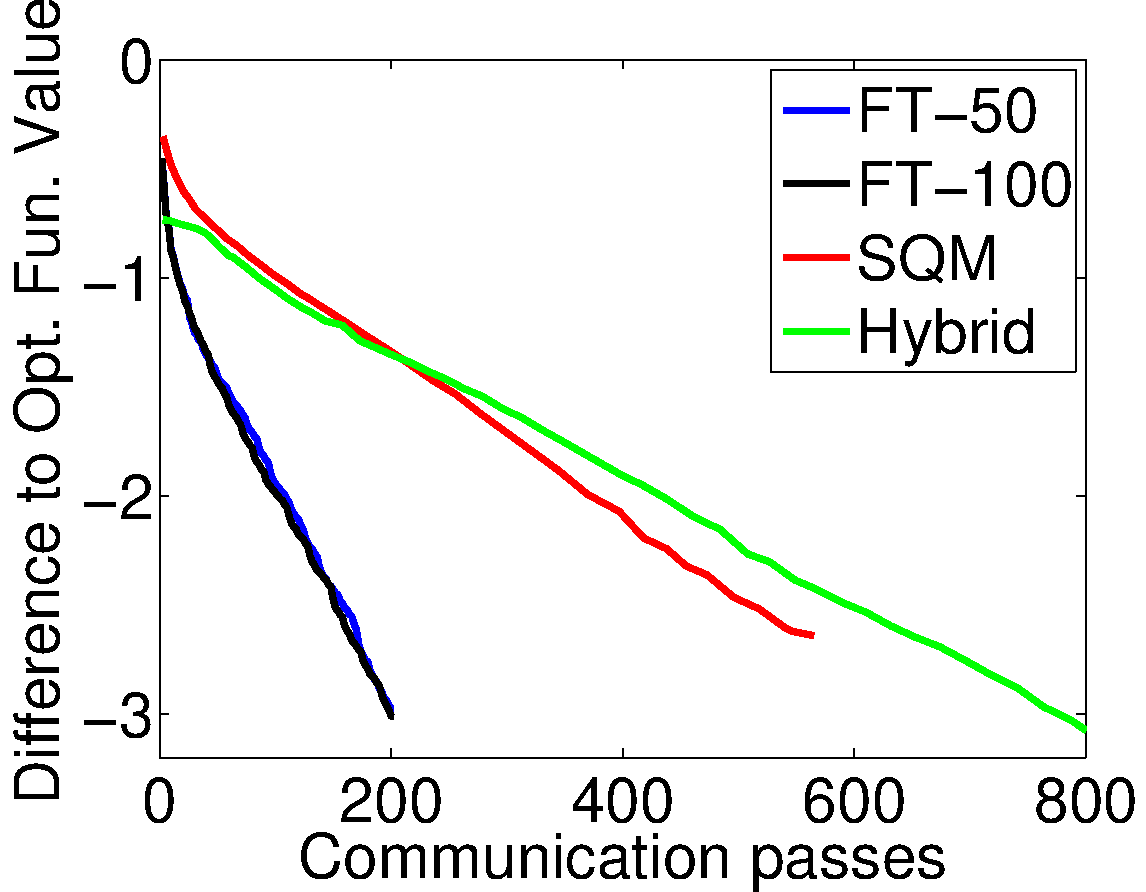
\includegraphics[width=0.46\linewidth]{figures/kddtron_100nodes_outeriters}
}
\subfigure[{\it{url}} - 6 nodes]{
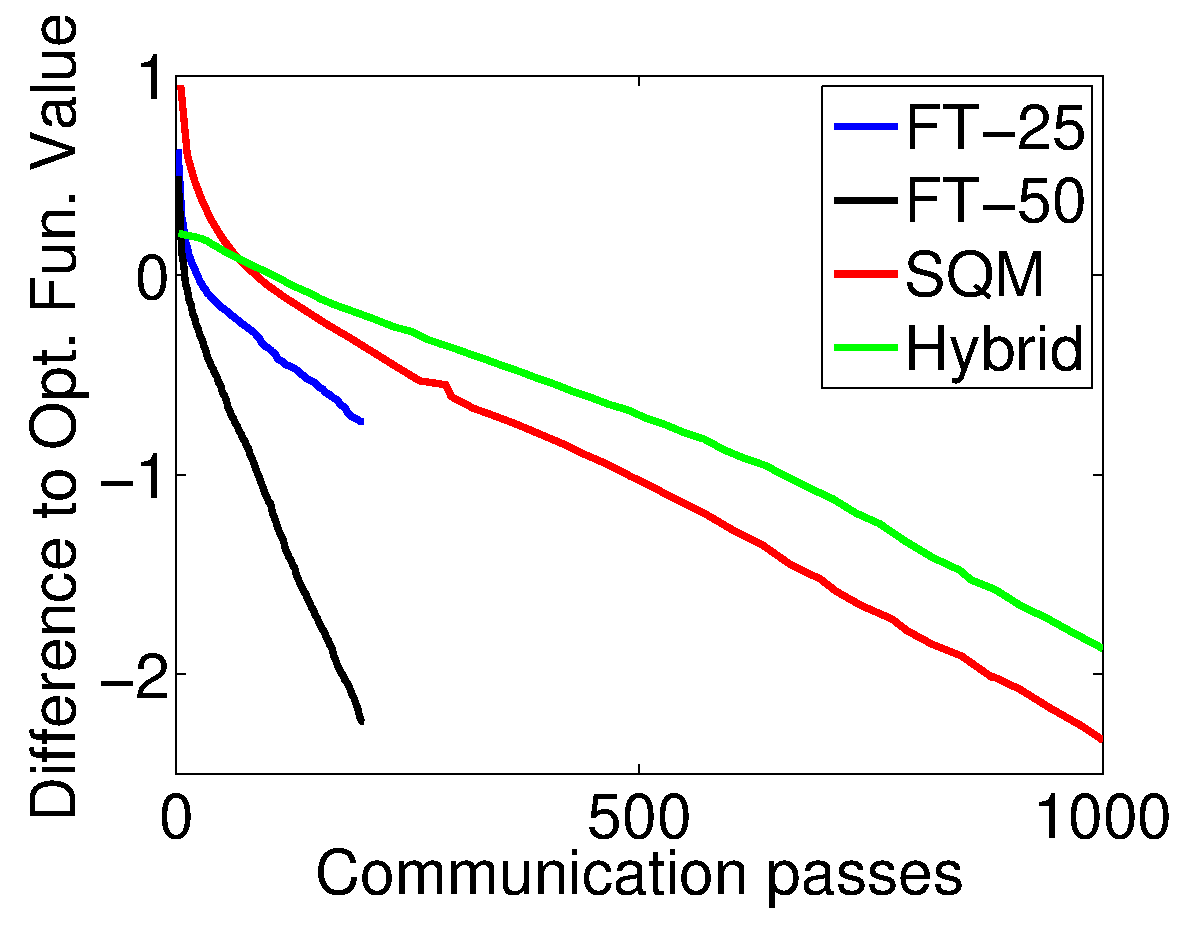
\includegraphics[width=0.46\linewidth]{figures/urltron_6nodes_outeriters}
}
\subfigure[{\it{url}} - 100 nodes]{
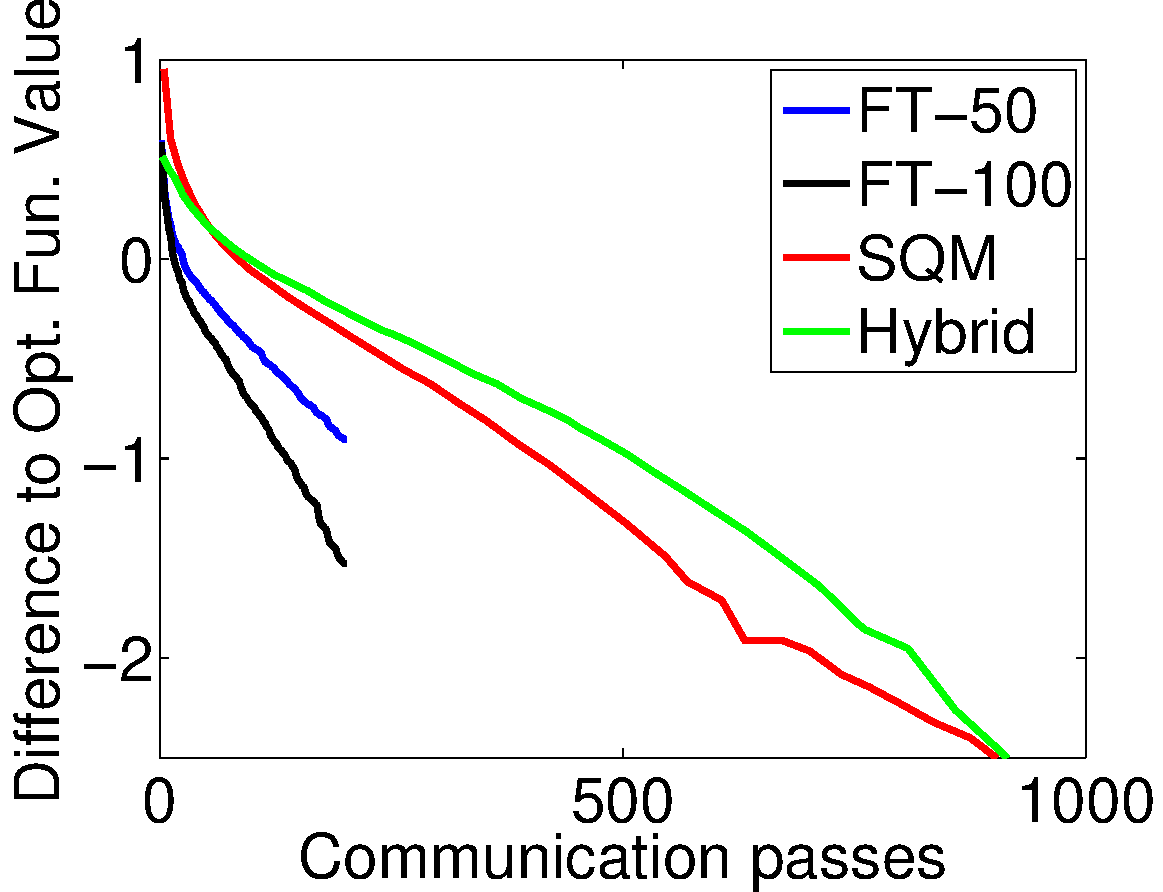
\includegraphics[width=0.46\linewidth]{figures/urltron_100nodes_outeriters}
}
\label{commpass}
\caption{Plots showing linear convergence of our method using TRON as the local optimizer. $x$-axis is the number of communication passes and $y$-axis is the relative
decrease in function value in $\log_{10}$ scale.}
\end{figure}

\subsection{Results}
{\bf{Linear Convergence. }}To validate linear convergence,  we study the variation of $(f-f^*)/f^*$ (in log scale) as a function of the number of communication passes\footnote{Note that we do not use the number of outer iterations as x-axis because it has different meaning for different methods. For example for {\it{SQM}} and {\it{HYBRID}} each outer iteration requires different number of passes (Hessian-vector computations) over data and hence different communication also. However, our class of methods requires fixed number of passes over data as well as only 2 communication passes per outer iteration.}, where $f^*$ is the optimal function value. (We obtained $f^*$ by running the algorithm to get a very accurate solution.) For our algorithms ({\it{FS-k}} and {\it{FT-k }}), the number of communication passes is just twice the number of outer iterations. From Figure 1, we make the following observations for {\it{FT-k }} on the {\it{kdd2010}} dataset: (a) the rate of convergence is linear for both $P=25$ and $100$, (b) it is steeper when $P=25$. This steeper behavior for $P=25$ is expected because the functional approximation in each node becomes better as the number of nodes decreases. Note that, almost always, the rate of convergence is better in the early stages of the optimization and becomes steady in the end stages. We observed similar linear convergence behavior for {\it{FS-k}} also. Note that the slope is dependent on $k$ and remains nearly same when $k$ is sufficiently large and the number of examples per node is small (see for example, the {\it{kdd2010}} dataset when $P=100$). Similar observations hold for the URL dataset as well. Overall, this experiment clearly demonstrates: (a) the flexibility of our distributed algorithm in using any linear convergent local optimization algorithm, (b) a linearly convergent IPM algorithm and (c) a parallel SGD method (with its variants such as SVRG).

%shows the results of number of communication passes versus the difference to the optimal function value for different number of nodes ($P=6,25,100$.  Note that both {\it{FS-k}} and {\it{FT-k }} show overall linear convergence (straight lines) for different values of $k$. As expected, the rate of convergence (slope) increases (with diminishing returns) as we increase $k$ since the local optimization becomes more accurate. It also increases with decreasing number of nodes $P$ as the functional approximation becomes better.

{\bf{Time Taken. }}Figure 2 shows the timing results. We observe that there is an optimum value of $k$ for which we get the best result. This is because although the rate of convergence becomes better with increasing $k$ (as discussed above), the computation cost starts increasing and becomes dominant after a certain value of $k$. Moreover, the optimal $k$ value also decreases with increasing $P$. This happens because of two reasons. First, the computation cost increases with decreasing number of nodes. As a result the number of inner iterations that we can perform before the computation cost starts dominating the communication cost, decreases. Second, since the functional approximation becomes better as $P$ decreases, we require lesser number of iterations to get a good descent direction. As a result, our approach does well even if $k$ is small. From our experiments, we also observed that at the optimal $k$, neither communication cost nor computation cost dominates other completely. Hence, as a rule of thumb, the value of $k$ should be chosen (or selected in a range) such that both the costs balance each other.
%{\bf{TRON vs. SVRG:}} TO be completed once results are there

%{\bf{Other Methods: }}Figures~\ref{},~\ref{}and~\ref{} compare our method with {\it{HYBRID}} and {\it{SQM}}. For {\it{FS-k}} we used $k=$ while for {\it{FT-k }} $k$ was set to.

\begin{figure}[t]
\centering
\subfigure[25 nodes]{
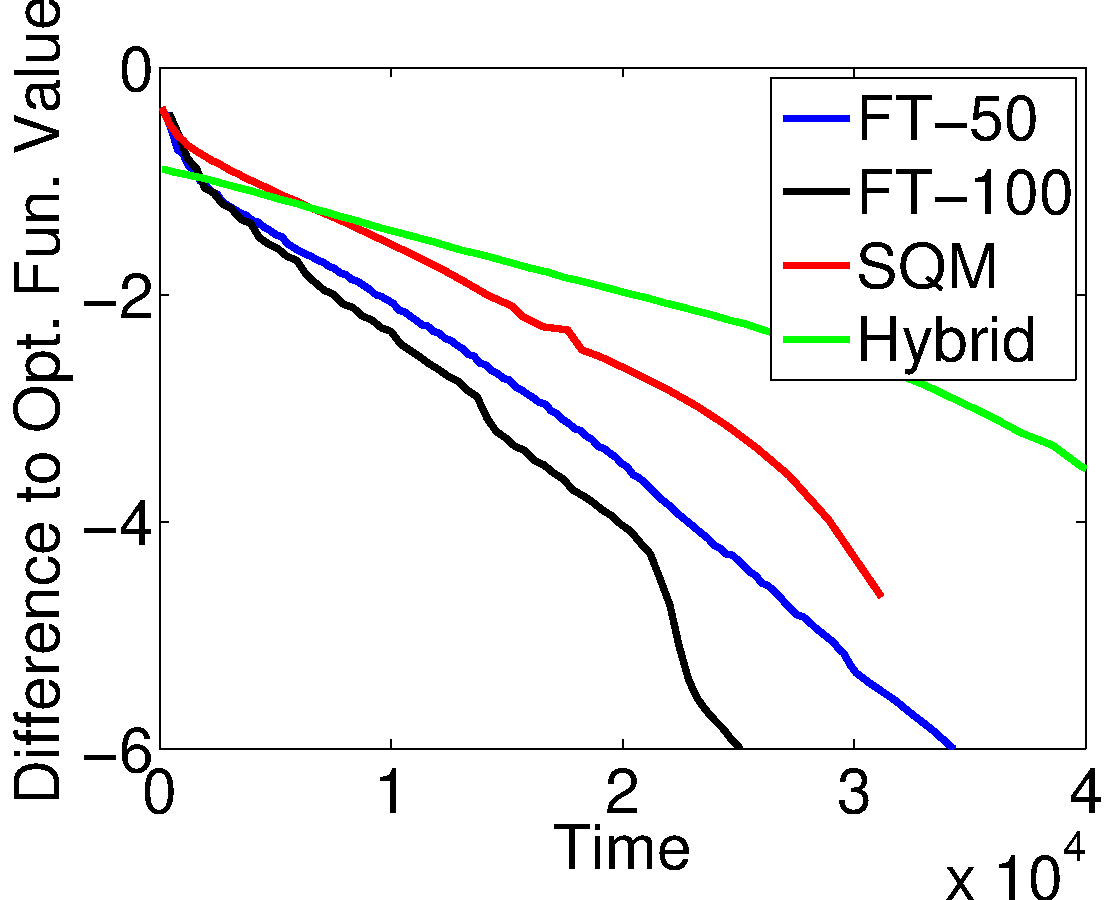
\includegraphics[width=0.46\linewidth]{figures/kddtron_25nodes_time}
}
\subfigure[100 nodes]{
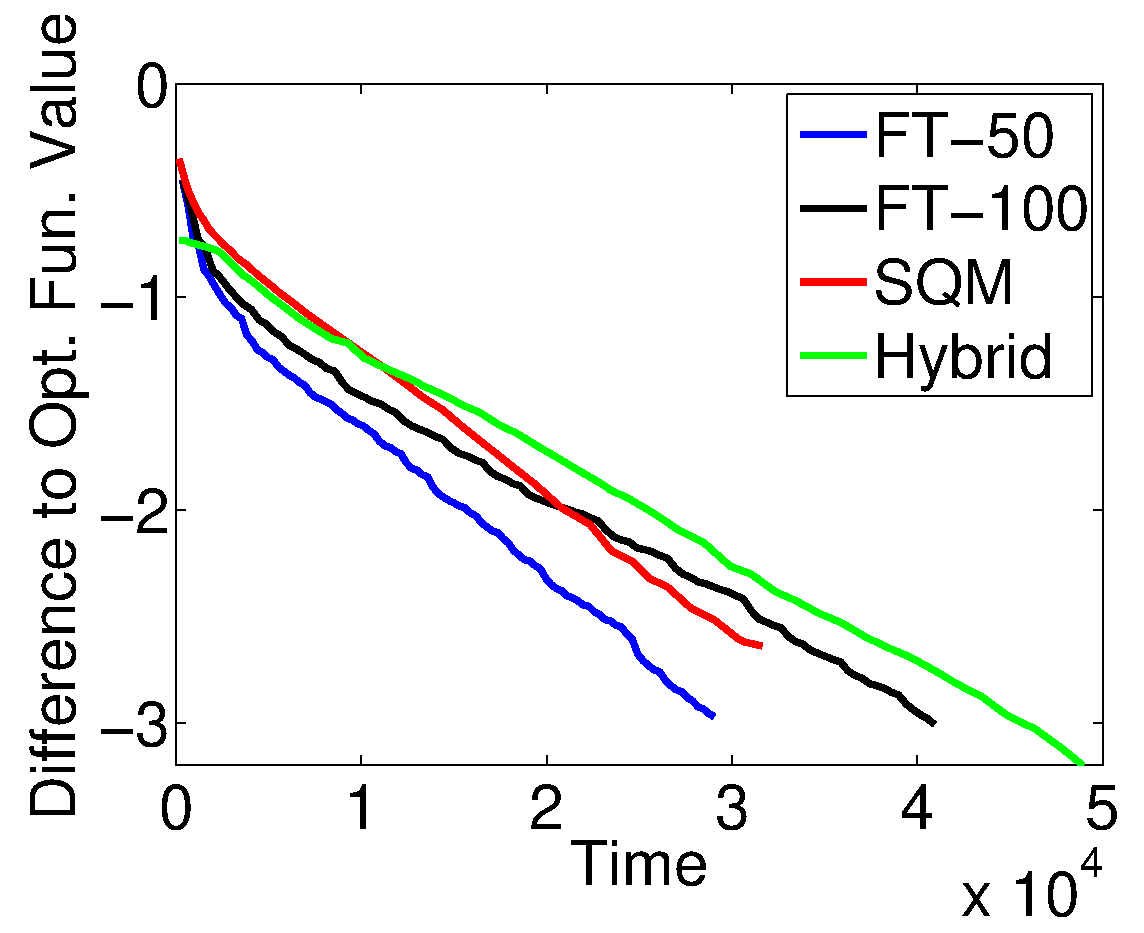
\includegraphics[width=0.46\linewidth]{figures/kddtron_100nodes_time}
}
\subfigure[25 nodes]{
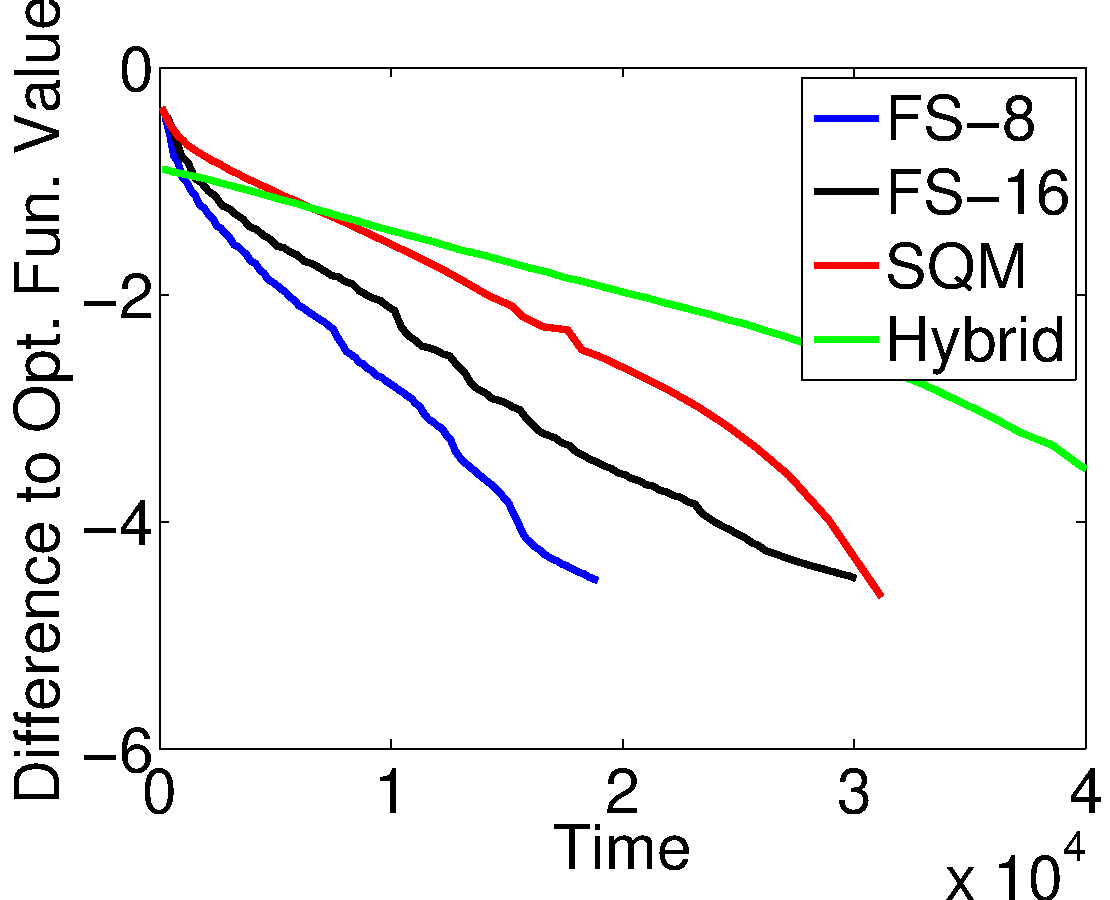
\includegraphics[width=0.46\linewidth]{figures/kddsvrg_25nodes_time}
}
\subfigure[100 nodes]{
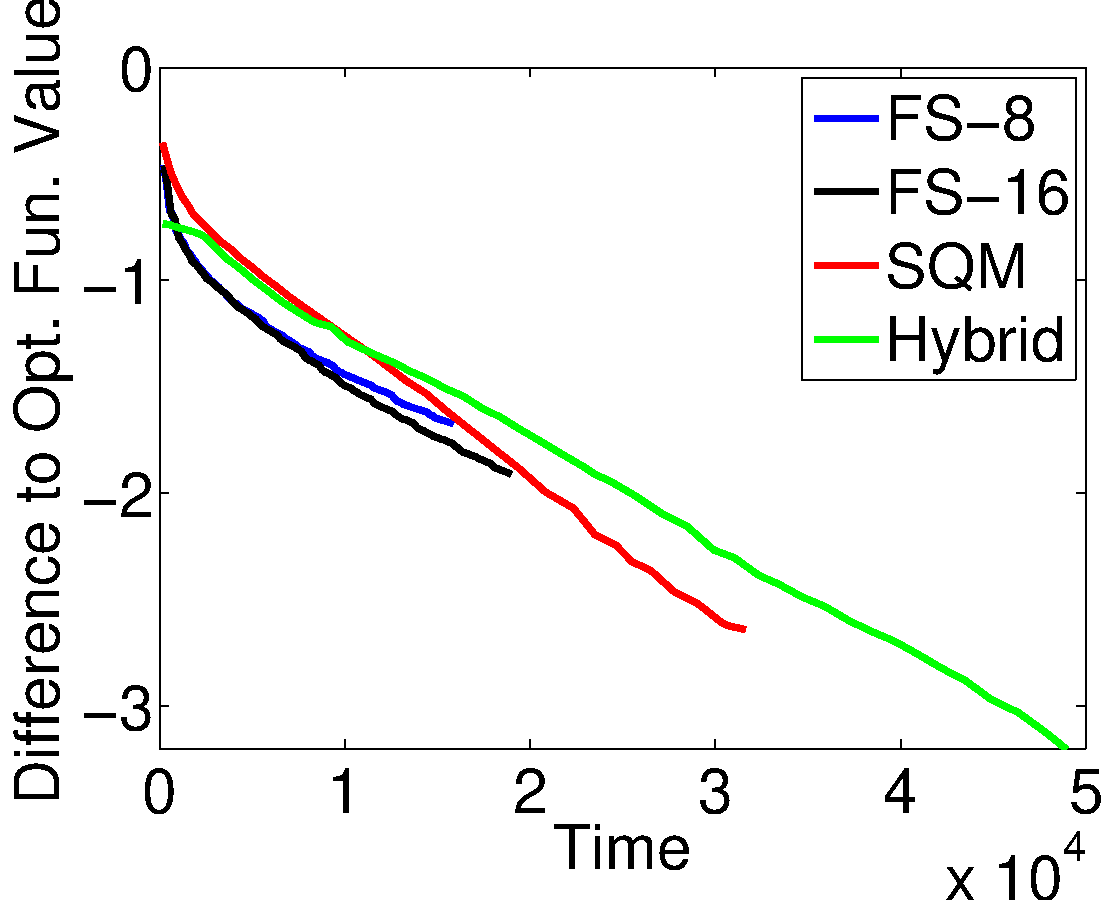
\includegraphics[width=0.46\linewidth]{figures/kddsvrg_100nodes_time}
}
\caption{Plots showing overall linear convergence of our method and comparisons with {\it{SQM}} and {\it{HYBRID}} for {\it{kdd2010}}. $x$-axis is time (in seconds). Results are shown using with TRON and SVRG for local optimization.}
\label{timepass}
\end{figure}

{\bf Comparison with other methods. }For {\it{HYBRID}} and {\it{SQM}} algorithms, the number of communication passes is equal to the number of Hessian-vector and gradient computations. From Figures 1 and 2, we first see that {\it{HYBRID}} performs better than {\it{SQM}} due to warm start when the number of iterations are small. However, the performance difference between {\it{HYBRID}} and {\it{SQM}} decreases with increasing iterations and eventually {\it{SQM}} performs better. This behavior is a bit surprising and needs to be investigated.

\comment{
{\bf Comparison with other methods. }For {\it{HYBRID}} and {\it{SQM}} algorithms, the number of communication passes is equal to the number of Hessian-vector and gradient computations. From Figures 1 and 2, we first see that {\it{HYBRID}} performs better than {\it{SQM}} due to warm start when the number of nodes is small. This is expected because we expect the local model weight vectors to be closer to the global one (as more data is available in each node). The performance difference between {\it{HYBRID}} and {\it{SQM}} decreases with increasing number of nodes as the variance among the local models increases. In fact, for {\it{kdd2010}}, {\it{HYBRID}} performed worse than {\it{SQM}} for $P=100$.
}
Second, both {\it{FS-k}} and {\it{FT-k }} need significantly less communication passes ($3-5$ times) than {\it{HYBRID}} to reach moderately small relative error (say $10^{-3}$). In this case, our algorithms perform better in terms of time also. Note that as seen in Figure 3, this is sufficient to get a good AUPRC performance; also, our algorithms (both {\it{FT-k }} and {\it{FS-k}}) reach the stable performance much quicker than other algorithms. This clearly illustrates the usefulness of our distributed algorithm when communication cost is the bottleneck.

One other important point to note is: {\it{HYBRID}} and {\it{SQM}} start performing better when a very small relative error (e.g., $10^{-6}$) is desirable. This behavior can be explained as follows: In the beginning of the optimization, our functional approximation gives a good global view to all the nodes. As a result, we perform better than {\it{SQM}} and {\it{HYBRID}} by doing multiple inner iterations on this global approximation. However, closer to the optimum, the function curvature starts dominating the rate of convergence. Since {\it{SQM}} and {\it{HYBRID}} have better curvature estimates (available via global Hessian) they start performing better near the optimal solution. Hence, in summary, our approach has good global convergence but slow local movement (i.e., near the optimal solution) while {\it{SQM}} and {\it{HYBRID}} have slow global convergence but good local movement. Although theoretically one can incorporate second order functional approximation in our approach also, effectively communicating the Hessian information can be challenging. In future, we would like to incorporate ideas from Quasi-newton algorithms like L-BFGS~\cite{liu89} in our functional approximation and develop hybrid algorithms that switch to {\it{SQM}} at some point in our method.

%We also notice that the gap between our methods and {\it{SQM}} and {\it{HYBRID}} decreases with increasing number of nodes. This happens because our functional approximation becomes cruder as $P$ increases. The exact $P$ up to which our approach performs better varies from dataset to dataset and depends on the learning curve. For steeper learning curves, our performance should degrade slower. The exact analysis is left as a future work. Similar observations can be made on the time curves in Figure~\ref{}.

%Finally, Figure~\ref{} shows time versus AUPRC results for different methods. Our method clearly outperforms both {\it{HYBRID}} and {\it{SQM}} in getting good AUPRC values (within $0.5\%$ of the optimal).

To conclude, our functional approximation based distributed learning algorithm is flexible and fills several gaps in the literature. We have demonstrated that our algorithms work well when (a) the number of features is very large, (b) the functional approximation is good, and (c) moderately small relative objective function error is desired. We expect to come up with better functional approximations and hybrid algorithms in the near future that does well under all conditions.





\begin{figure}
\centering
\subfigure[25 nodes]{
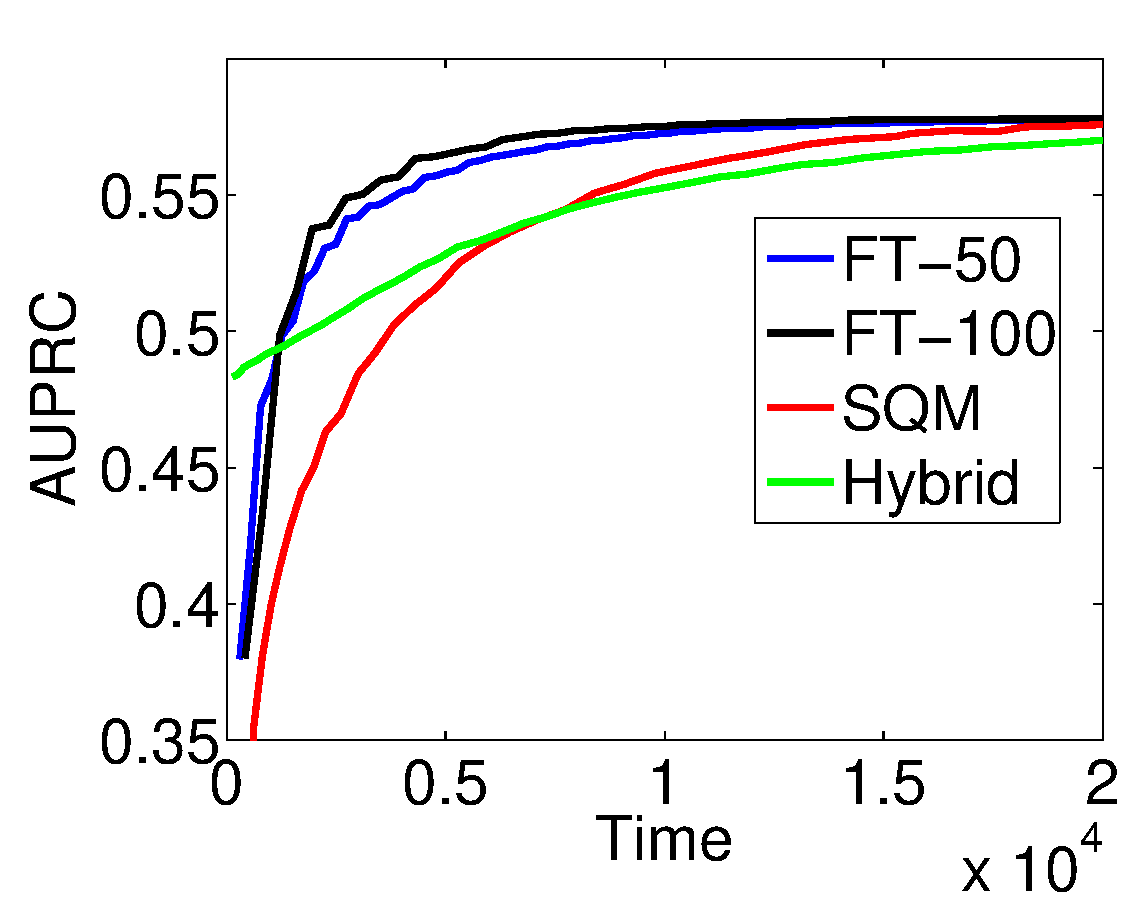
\includegraphics[width=0.46\linewidth]{figures/kddtron_25nodes_auprc}
}
\subfigure[100 nodes]{
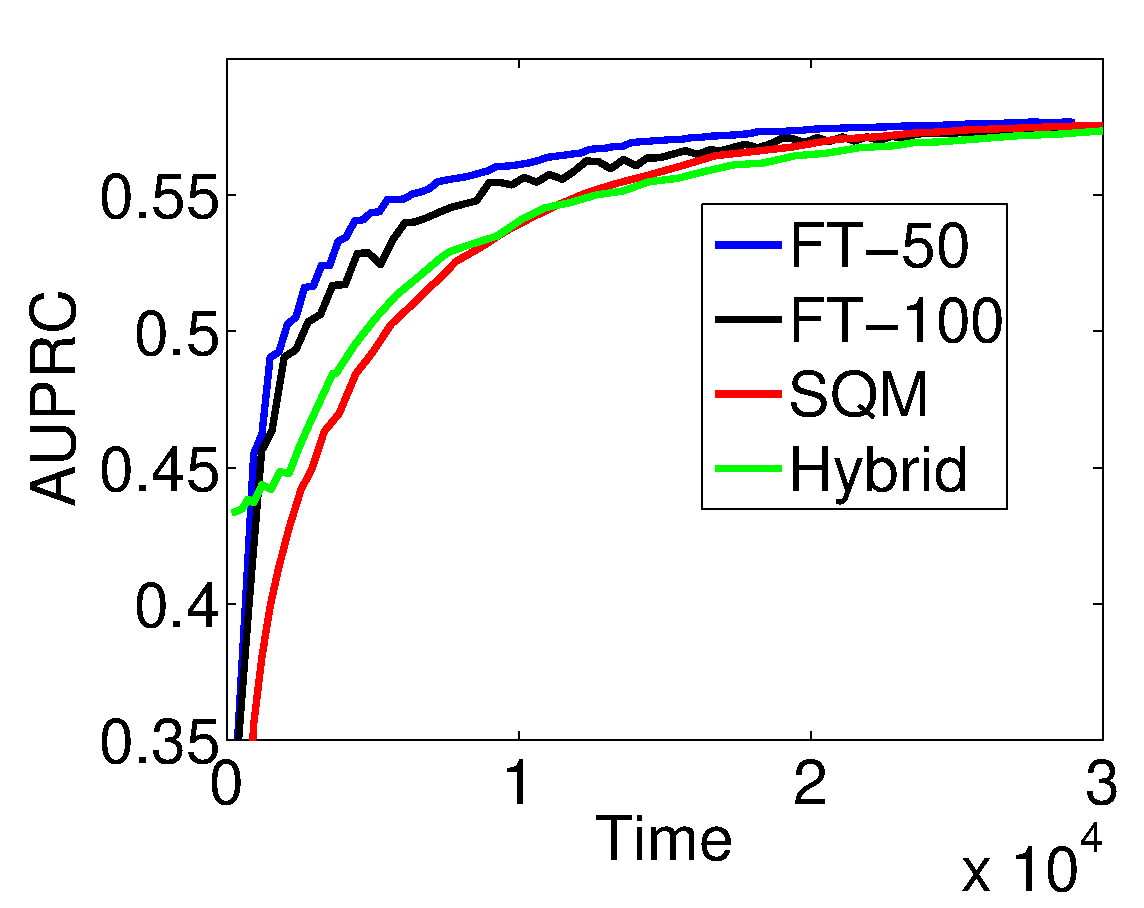
\includegraphics[width=0.46\linewidth]{figures/kddtron_100nodes_auprc}
}
\subfigure[25 nodes]{
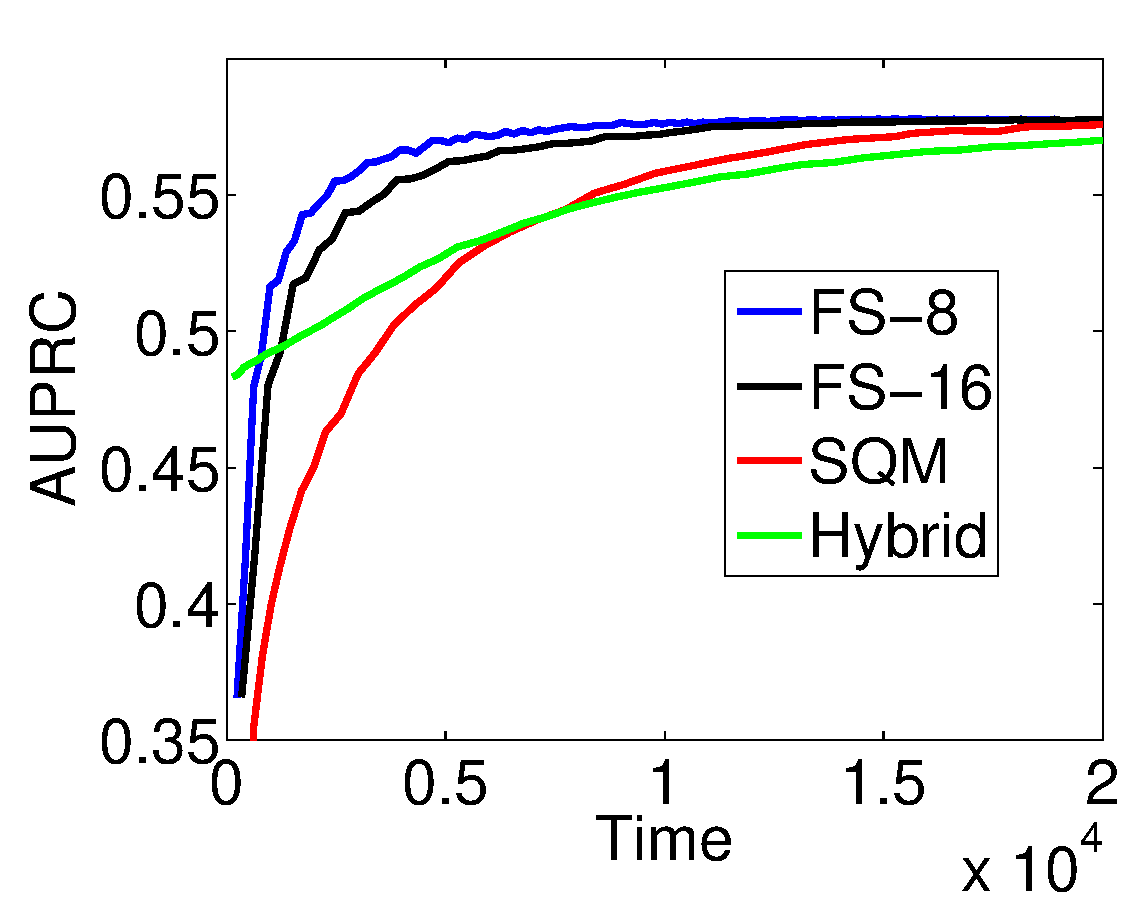
\includegraphics[width=0.46\linewidth]{figures/kddsvrg_25nodes_auprc}
}
\subfigure[100 nodes]{
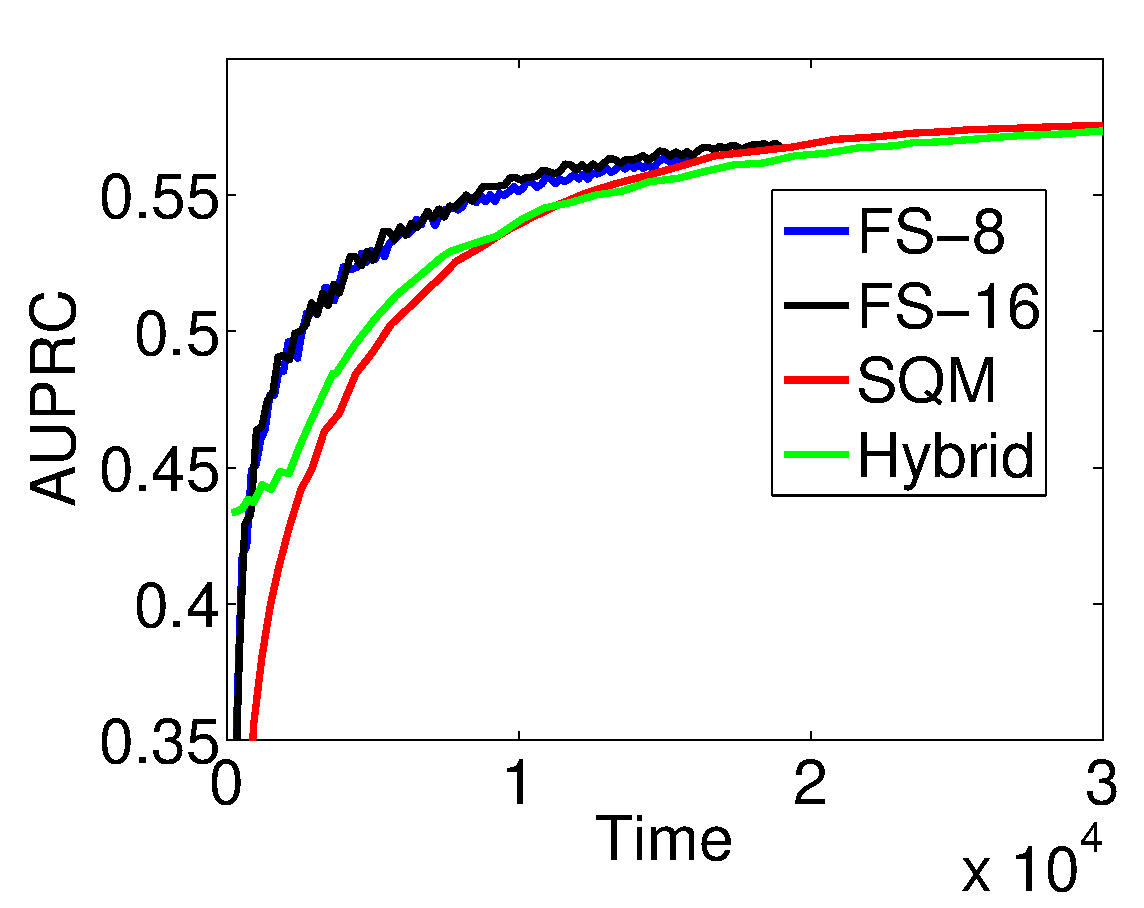
\includegraphics[width=0.46\linewidth]{figures/kddsvrg_100nodes_auprc}
}
\caption{Plots showing AUPRC metric for our method, {\it{SQM}} and {\it{HYBRID}} for {\it{kdd2010}}. $x$-axis is time (in seconds).}
\label{auprc}
\end{figure}


\section{Discussion}
\label{disc}

In this section, we discuss briefly, other different distributed settings made possible by our algorithm. The aim is to show the flexibility and generality of our approach while ensuring {\it glrc}.\comment{ We will also talk briefly about the extension to non-convex setting.}

Section~\ref{distr} considered example partitioning where examples are distributed across the nodes. First, it is worth mentioning that, due to the gradient consistency condition, {\it partitioning} is not a necessary constraint; our theory allows examples to be resampled, i.e., each example is allowed to be a part of any number of nodes arbitrarily. For example, to reduce the number of outer iterations, it helps to have more examples in each node.

Second, the theory proposed in section~\ref{distr} holds for feature partitioning also. Suppose, in each node $p$ we restrict ourselves to a subset of features, $J_p\subset \{1,\ldots,d\}$, i.e., include the constraint,
$w_p \in  \{ w: w(j)=w^r(j) \;\; \forall r\not\in J_p\}$,
where $w(j)$ denotes the weight of the $j^{th}$ feature. Note that we do not need $\{J_p\}$ to form a partition. This is useful since important features can be included in all the nodes.

{\bf Gradient sub-consistency.} Given $w^r$ and $J_p$ we say that $\fhat_p(w)$ has gradient sub-consistency with $f$ at $w^r$ on $J_p$ if $\frac{\partial f}{\partial w(j)} (w^r) = \frac{\partial \fhat}{\partial w(j)} (w^r) \;\; \forall \; j\in J_p$.

Under the above condition, we can modify the algorithm proposed in Section~\ref{distr} to come up with a feature decomposition algorithm with {\it glrc}.

Several feature decomposition based approaches~\cite{richtarik2013,patriksson1998fp} have been proposed in the literature. The one closest to our method is the work by Patrikkson on a synchronized parallel algorithm~\cite{patriksson1998fp} which extends a generic cost approximation algorithm~\cite{patriksson1998ca} that is similar to our functional approximation. The sub-problems on the partitions are solved in parallel. Although the objective function is not assumed to be convex, the cost approximation is required to satisfy a monotone property, implying that the approximation is convex. The algorithm only has asymptotic linear rate of convergence and it requires the feature partitions to be disjoint. In contrast, our method has {\it glrc} and works even if features overlap in partitions. Moreover, there does not exist any counterpart of our example partitioning based distributed algorithm discussed in section~\ref{distr}.

Our approach can be easily generalized to joint example-feature partitioning as well as non-convex setting. The exact details of all the extensions mentioned above and related experiments are left for future work.

\section{Conclusion}
To conclude, we have proposed a novel functional approximation based distributed algorithm with provable global linear rate of convergence. The algorithm is general and flexible in the 
sense of allowing different local approximations at the node level, different algorithms for optimizing the local approximation, early stopping and general data usage in the nodes.

\section{Appendix A: Proofs}
\label{proofs}

\subsection{Proofs of the results in section~\ref{general}}

Let us now consider the establishment of the convergence theory given in section~\ref{general}.

{\bf Proof of Lemma 1.}
Let $\rho(t)=f(w^r+td^r)$ and $\gamma(t)=\rho(t)-\rho(0)-\alpha t\rho^\prime(0)$.
Note the following connections with quantities involved in Lemma 1: $\rho(t)=f^{r+1}$, $\rho(0)=f^r$, $\rho^\prime(t)=g^{r+1}\cdot d^r$ and $\gamma(t)=f^{r+1} - f^r - \alpha g^r\cdot(w^{r+1}-w^r)$.
(\ref{ag}) corresponds to the condition $\gamma(t)\le 0$ and (\ref{wolfe}) corresponds to the condition $\rho^\prime(t)\ge \beta\rho^\prime(0)$.

$\gamma^\prime(t) = \rho^\prime(t)-\alpha \rho^\prime(0)$.
$\rho^\prime(0)<0$.
$\rho^\prime$ is strictly monotone increasing because, by assumption A2,
\begin{equation}
\rho^\prime(t)-\rho^\prime(\ttilde) \ge \sigma (t-\ttilde)\|d^r\|^2 \;\; \forall \; t, \ttilde
\label{prop11}
\end{equation}
This implies that $\gamma^\prime$ is also strictly monotone increasing and, all four, $\rho$, $\rho^\prime$, $\gamma^\prime$ and $\gamma$ tend to infinity as $t$ tends to infinity.

Let $t_\beta$ be the point at which $\rho^\prime(t)=\beta\rho^\prime(0)$. Since $\rho^\prime(0)<0$ and $\rho^\prime$ is strictly monotone increasing, $t_\beta$ is unique and $t_\beta>0$. This validates the definition in (\ref{tbeta}). Monotonicity of $\rho^\prime$ implies that (\ref{wolfe}) is satisfied iff $t\ge t_\beta$.

Note that $\gamma(0)=0$ and $\gamma^\prime(0)<0$. Also, since $\gamma^\prime$ is monotone increasing and $\gamma(t)\to\infty$ as $t\to\infty$, there exists a unique $t_\alpha>0$ such that $\gamma(t_\alpha)=0$, which validates the definition in (\ref{talpha}). It is easily checked that $\gamma(t)\le 0$ iff $t\in [0,t_\alpha]$.

The properties also imply $\gamma^\prime(t_\alpha)> 0$, which means $\rho^\prime(t_\alpha) \ge \alpha\rho^\prime(0)$. By the monotonicity of $\rho^\prime$ we get $t_\alpha>t_\beta$, proving the lemma.


{\bf Proof of Theorem 2.} Using (\ref{wolfe}) and A1,
\begin{equation}
(\beta-1)g^r\cdot d^r \le (g^{r+1}-g^r)\cdot d^r \le Lt\|d^r\|^2
\label{th21}
\end{equation}
This gives a lower bound on $t$:
\begin{equation}
t \ge \frac{(1-\beta)}{L\|d^r\|^2} (-g^r\cdot d^r)
\label{th22}
\end{equation}
Using (\ref{ag}), (\ref{th22}) and (\ref{angle}) we get
\begin{eqnarray}
f^{r+1} & \le & f^r + \alpha t g^r\cdot d^r \nonumber \\
        & \le & f^r - \frac{\alpha(1-\beta)}{L\|d^r\|^2} (-g^r\cdot d^r)^2 \nonumber \\
        & \le & f^r - \frac{\alpha(1-\beta)}{L} \cos^2 \theta \|g^r\|^2
\label{th23}
\end{eqnarray}
Subtracting $f^\star$ gives
\begin{equation}
(f^{r+1} - f^\star) \le  (f^r-f^\star) - \frac{\alpha(1-\beta)}{L} \cos^2 \theta \|g^r\|^2
\label{th24}
\end{equation}
A2 together with $g(w^\star)=0$ implies $\|g^r\|^2\ge\sigma^2\|w^r-w^\star\|^2$. Also A1 implies $f^r-f^\star \le \frac{L}{2}\|w^r-w^\star\|^2$~\cite{smola2008}. Using these in (\ref{th24}) gives
\begin{eqnarray}
(f^{r+1}-f^\star) & \le & (f^r - f^\star) - 2\alpha(1-\beta)\frac{\sigma^2}{L^2} \cos^2\theta (f^r - f^\star) \nonumber \\
                  & \le & (1 - 2\alpha(1-\beta)\frac{\sigma^2}{L^2} \cos^2\theta) (f^r - f^\star)
\label{th25}
\end{eqnarray}
Let $\delta = (1 - 2\alpha(1-\beta)\frac{\sigma^2}{L^2} \cos^2\theta)$. Clearly $0 < \delta < 1$. Theorem 2 follows.

\subsection{Proofs of the results in section~\ref{distr}}

Let us now consider the establishment of the convergence theory given in section~\ref{distr}. We begin by establishing that the exact minimizer of $\fhat_p$ makes a sufficient angle of descent at $w^r$.

{\bf Lemma 5.} Let $\what_p^\star$ be the minimizer of $\fhat_p$. Let $d_p= (\what_p^\star-w^r)$. Then
\begin{equation}
-g^r\cdot d_p \ge (\sigma/L) \|g^r\| \|d_p\|
\label{suffangle}
\end{equation}

{\bf Proof.} First note, using gradient consistency and $\grad f_p(\what_p^\star)=0$ that
\begin{equation}
\|g^r\| = \| \grad \fhat_p(w^r)-\grad \fhat_p(\what_p^\star) \| \le L\|d_p\|
\label{lem211}
\end{equation}
Now,
\begin{eqnarray}
-g^r\cdot d_p &=&(\grad \fhat_p(w^r)-\grad \fhat_p(\what_p^\star))^T(w^r-\what_p^\star) \nonumber \\
            &\ge& \sigma \|d_p\|^2 \nonumber \\
            &=& \sigma \|g^r\| \|d_p\| \frac{\|d_p\|}{\|g^r\|} \nonumber \\
            &\ge& \frac{\sigma}{L} \|g^r\| \|d_p\|
\label{lem212}
\end{eqnarray}
where the second line comes from $\sigma$-strong convexity and the fourth line follows from (\ref{lem211}).

{\bf Proof of Lemma 3.}
Let us now turn to the question of approximate stopping and establish Lemma 3. Given $\theta$ satisfying (\ref{thetadef}) let us choose $\zeta\in (0,1)$ such that
\begin{equation}
\label{lem2211}
\frac{\pi}{2} > \theta > \cos^{-1} \frac{\sigma}{L} + \cos^{-1} \zeta
\end{equation}

%{\bf Lemma 7.} Assume $g(w^r)\not=0$. Suppose we minimize $\fhat_p$ using an optimizer that starts from $v^0=w^r$ and generates a sequence $\{v^k\}$ having linear convergence, i.e.,
%\begin{equation}
%\fhat_p(v^{k+1}) - \fhat_p^\star \le \delta (\fhat_p(v^k) - \fhat_p^\star)
%\label{22a}
%\end{equation}
%where $\fhat_p^\star = \fhat_p(\what_p^\star)$. Then, given any $\zeta$ satisfying $0<\zeta<1$, there exists $\khat$ (which depends only on $\zeta$, $\sigma$ and $L$) such that
%\begin{equation}
%\cos \phi^k \ge \zeta \;\; \forall k\ge \khat
%\label{22b}
%\end{equation}
%where $\phi^k$ is the angle between $\what_p^\star-w^r$ and $v^k-w^r$.

%fhat to fhat_p

%Add a diagram to help
\begin{figure}
\begin{center}
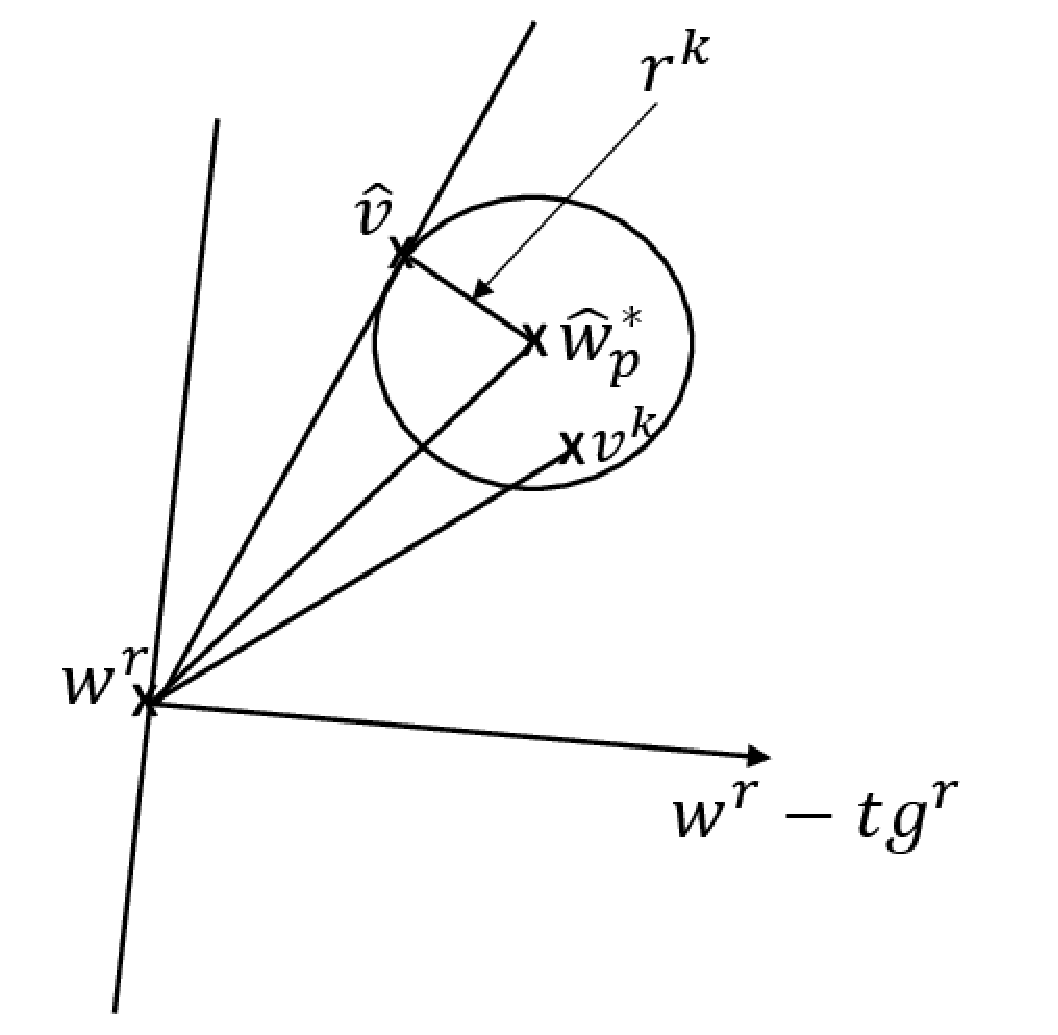
\includegraphics[width=0.8\columnwidth]{figures/spherefig}
\caption{Construction used in the proof of Lemma 3.}
\end{center}
\label{spherefig}
\end{figure}


By A3 and equations ($3.16$) and ($3.22$) in~\cite{smola2008}, we get
\begin{equation}
\frac{\sigma}{2} \|v-\what_p^\star\|^2 \le \fhat_p(v) - \fhat_p^\star \le \frac{L}{2} \|v-\what_p^\star\|^2
\label{lem221}
\end{equation}
After $k$ iterations we have
\begin{equation}
\fhat_p(v^k) - \fhat_p^\star \le \delta^k (\fhat_p(w^r) - \fhat_p^\star)
\label{lem222}
\end{equation}
We can use these to get
\begin{eqnarray}
\|v^k-\what_p^\star\|^2 &\le& \frac{2(\fhat_p(v^k)-\fhat_p^\star)}{\sigma} \nonumber \\
                        &\le& \frac{2\delta^k (\fhat_p(w^r)-\fhat_p^\star)}{\sigma} \nonumber \\
                        &\le& \frac{\delta^kL}{\sigma} \|w^r-\what_p^\star\|^2 \defs (r^k)^2
\label{lem223}
\end{eqnarray}
For now let us assume the following:
\begin{equation}
\|v^k-\what_p^\star\|^2 \le \|w^r-\what_p^\star\|^2
\label{lem224}
\end{equation}
Using (\ref{lem223}) note that (\ref{lem224}) holds if
\begin{equation}
\frac{\delta^kL}{\sigma} \le 1
\label{lem225}
\end{equation}
Let $S^k$ be the sphere, $S^k = \{ v : \|v-\what_p^\star\|^2 \le (r^k)^2 \}$. By (\ref{lem223})
%and (\ref{lem224})
we have $v^k\in S^k$. See Figure~\ref{spherefig}. Therefore,
\begin{equation}
\phi^k \le \max_{v\in S^k} \phi(v)
\label{lem226}
\end{equation}
where $\phi^k$ is the angle between $\what_p^\star-w^r$ and $v^k-w^r$, and $\phi(v)$ is the angle between $v-w^r$ and $\what_p^\star-w^r$. Given the simple geometry, it is easy to see that $\max_{v\in S^k} \phi(v)$ is attained by a point $\vhat$ lying on the boundary of $S^k$ (i.e., $\|\vhat-\what_p^\star\|^2 = (r^k)^2$) and satisfying $(\vhat-\what_p^\star)\perp (\vhat-w^r)$. This geometry yields
\begin{eqnarray}
\cos^2 \phi(\vhat) &=& \frac{\|\vhat-w^r\|^2}{\|\what_p^\star-w^r\|^2} \nonumber \\
                   &=& \frac{\|\what_p^\star-w^r\|^2-(r^k)^2}{\|\what_p^\star-w^r\|^2} \nonumber \\
                   &=& 1-\frac{(r^k)^2}{\|\what_p^\star-w^r\|^2} = 1-\frac{\delta^kL}{\sigma}
\label{lem227}
\end{eqnarray}
Since $\phi^k\le \phi(\vhat)$,
\begin{equation}
\cos^2 \phi^k \ge 1-\frac{\delta^kL}{\sigma}
\label{lem228}
\end{equation}
Thus, if
\begin{equation}
1-\frac{\delta^kL}{\sigma} \ge \zeta^2
\label{lem229}
\end{equation}
then
\begin{equation}
\cos \phi^k \ge \zeta \;\; \forall k\ge \khat
\label{22b}
\end{equation}
holds. By (\ref{lem2211}) this yields $\phase{-g^r,v^k-w^r} \le \theta$, the result needed in Lemma 3. Since $\zeta>0$, (\ref{lem229}) implies (\ref{lem225}), so (\ref{lem224}) holds and there is no need to separately satisfy it. Now (\ref{lem229}) holds if
\begin{equation}
k \ge \khat \defs \frac{\log (L/(\sigma(1-\zeta^2)))}{\log(1/\delta)}
\label{lem2210}
\end{equation}
which proves the lemma.

{\bf Proof of Theorem 4.} It trivially follows from a combination of Lemma 3 and Theorem 2.


\def\C{C}
\def\Ccomp{C^{\rm Comp}}
\def\Ccomm{C^{\rm Comm}}
\def\Csqm{C_{\rm SQM}}
\def\Csvrg{C_{\rm SVRG}}
\def\Ccompsqm{C^{\rm Comp}_{\rm SQM}}
\def\Ccommsqm{C^{\rm Comm}_{\rm SQM}}
\def\Ccompsvrg{C^{\rm Comp}_{\rm SVRG}}
\def\Ccommsvrg{C^{\rm Comm}_{\rm SVRG}}
\def\Tout{T^{\rm outer}}
\def\Tin{T^{\rm inner}}
\def\Toutsqm{T^{\rm outer}_{\rm SQM}}
\def\Toutsvrg{T^{\rm outer}_{\rm SVRG}}

\section{Appendix B: Complexity analysis}
\label{proofs}
Let us use the notations of section~\ref{distr} given around (\ref{comm}). We define the overall cost of any distributed algorithm as
\begin{eqnarray}
[(c_1\frac{nz}{p} + c_2m)\Tin + c_3 \gamma m \log_2 P]\Tout,
\label{costanal}
\end{eqnarray}
where $\Tout$ is the number of outer iterations, $\Tin$ is the number of inner iterations at each node before communication happens and  $c_1$ and $c_2$ denote the number of passes over the data and $m$-dimensional dot products per inner iteration respectively. For communication, we assume an AllReduce binary tree as described in Agarwal et al~\yrcite{agarwal2011} without pipelining. As a result, we get a multiplicative factor of $log_2 P$ in our cost. $\gamma$ is the ratio of computation to communication speed. For sparse datasets $\gamma$ is very large. $c_3$ is the number of $m$-dimensional vectors (gradients, Hessian-vector computations etc.) we need to communicate.

\begin{table}[ht]
\caption{Value of cost parameters} % title of Table
\centering % used for centering table
\begin{tabular}{c c c c c c c} % centered columns (4 columns)
\hline\hline %inserts double horizontal lines
Method & $c_1$ & $c_2$ & $c_3$ & $\Tin$ \\ %[0.5ex] % inserts table
%heading
\hline
SQM & $2$ & $\approx 5-10$ & $1$ & $1$ \\
Our & $1.2$ & $0.2$ & $2$ & $\hat{k}$ \\
\hline
\end{tabular}
\label{tab:params}
\end{table}

The values of different parameters for $SQM$ implemented using TRON and our approach implemented using SVRG are given in Table~\ref{tab:params}. $\Toutsqm$ is the number of overall conjugate gradient iterations plus gradient computations.

Since dense dot products are extremely fast and $c_3$ is a small number for both the approaches, we ignore it for simplicity. Now for our method to have lesser cost than $SQM$, we can use (\ref{costanal}) to get the condition,
%we need $\Csvrg \leq \Csqm$. Plugging in the parameter values and rearranging,
\begin{equation}
(1.2\hat{k}\Toutsvrg - 2\Toutsqm)\frac{nz}{P}  \leq  (\Toutsqm - 2 \Toutsvrg) \gamma m \log_2 P
\end{equation}
Ignoring $\Toutsqm$ on the left side of this inequality and rearranging, we get the looser condition,
\begin{equation}
\frac{nz}{m}  \leq  \frac{\gamma P\log_2 P}{\hat{k}} \frac{1}{1.2}(\frac{\Toutsqm}{\Toutsvrg} - 2 )
\end{equation}
Assuming $\Toutsqm > 3.2\Toutsvrg$, we arrive at the final condition in equation~(\ref{comm}). 
%Note that in our experiments (section~\ref{distr}), the savings we get in the outer iterations is typically more than the factor $3.2$.



\bibliography{falda}
\bibliographystyle{icml2014}



\end{document}
